 \باب{بوولین الجبرا}
بوولین الجبرا انگلستان کے   ریاضی  دان جارج بوولی کے نام سے جانا جاتا  ہے، جنہوں نے اس الجبرا کو دریافت کیا۔بوولین الجبرا ذہنی سوچ یعنی منطق کو الجبرائی روپ  میں لکھنے کی صلاحیت رکھتی ہے۔اس لئے  حیرانی کی بات نہیں کہ  کمپیوٹر اسی کو استعمال کرتا ہے۔

\حصہ{بوولین الجبرا کے بنیادی تصورات} \شناخت{حصہ_بوولین_الجبرا_بنیادی_تصورات}
عام الجبرا میں متغیرات استعمال کرتے  ہوئے  تصور کیا جاتا ہے کہ ان کی  قیمت کچھ بھی  ہو سکتی ہے۔مثلاً،  تفاعل   \عددی{z=f(x,y)}،  جہاں   \عددی{x} اور  \عددی{y}  آزاد متغیرات   جبکہ \عددی{z}  تابع متغیر ہے،  میں متغیرات کی چند   ممکنہ قیمتیں درج ذیل     ہیں۔
\begin{center}
\begin{otherlanguage}{english}
\begin{tabular}{CC|C}
\toprule
x&y&z\\
\midrule
0&0&0\\
1&2&5\\
2&1&4\\
3&2&7\\
2&2&6\\
3&1&5\\
\bottomrule
\end{tabular}
\end{otherlanguage}
\end{center}
اس تفاعل جس  کو ایک نا مکمل جدول کے روپ میں  پیش کیا گیا ہے  کا الجبرائی روپ   درج ذیل ہے۔
 \begin{align*}
 z=x+2y
 \end{align*}
اس کے برعکس،  بوولین الجبرا میں متغیرات کی صرف دو ممکنہ قیمتیں ہیں۔ ان دو قیمتوں کو عموماً   \عددی{0} (صفر)    اور   \عددی{1} (ایک)   سے ظاہر کیا جاتا ہے۔بوولین تفاعل کی چند مثالوں پر غور کرتے ہیں۔

\جزوحصہ{منطقی ضرب}
تصور کریں  \عددی{X}  اور \عددی{Y}  آزاد بوولین متغیرات ہیں،  جبکہ \عددی{Z}  ان کا تابع بوولین متغیر \عددی{Z=f(X,Y)} ہے۔ چونکہ \عددی{X}  بوولین متغیر ہے،  لہٰذا اس کی ممکنہ قیمتیں صرف \عددی{0} اور \عددی{1} ہیں۔اسی طرح \عددی{Y}  بھی بوولین متغیر ہے،  لہٰذا اس کی قیمت  بھی صرف  \عددی{0} اور \عددی{1} ہو سکتی ہے۔تابع متغیر \عددی{Z}بھی بوولین متغیر ہے۔اس طرح اگرچہ اس کی قیمت \عددی{X} اور \عددی{Y} کی تابع ہے،   اس کے باوجود \عددی{Z} کی قیمت  صرف  \عددی{0} یا \عددی{1}    ہی ہو سکتا ہے۔ متغیرات \عددی{X} اور \عددی{Y}  درج ذیل چار ممکنہ ترتیب میں پائے جا سکتے ہیں۔
\begin{center}
\begin{otherlanguage}{english}
\begin{tabular}{CC}
\toprule
X&Y\\
\midrule
0&0\\
0&1\\
1&0\\
1&1\\
\bottomrule
\end{tabular}
\end{otherlanguage}
\end{center}
ان چار ممکنہ صورتوں میں \عددی{Z} کی   قیمت \عددی{0} یا \عددی{1}  ہوگی۔

آئیں، جدول \حوالہ{جدول_بوولین_جمع} میں پیش کیے گئے منطقی تفاعل پر غور کرتے ہیں جس کی تمام ممکنہ قیمتیں اس جدول میں دی گئی ہیں۔
\begin{table}
\centering
\begin{otherlanguage}{english}
\begin{tabular}{CC|C}
\toprule
X&Y&Z\\
\midrule
0&0&0\\
0&1&0\\
1&0&0\\
1&1&1\\
\bottomrule
\end{tabular}
\end{otherlanguage}
\caption{دو   متغیر منطقی ضرب}
\label{جدول_بوولین_جمع}
\end{table}
اس مثال میں تابع متغیر \عددی{Z}   کی قیمت صرف   اس وقت   \عددی{1}  ہے جب \عددی{X}   اور \عددی{Y}  دونوں کی قیمت \عددی{1}   ہے۔یہی قیمتیں \عددی{X}  اور \عددی{Y}  کی سادہ ضرب \عددی{X\cdot Y}  سے بھی حاصل ہوتی ہیں (ذیل دیکھیں)۔
\begin{align*}
0\cdot 0&=0\\
0\cdot 1&=0\\
1\cdot 0&=0\\
1\cdot 1&=1
\end{align*}
اسی کی بنا پر جدول \حوالہ{جدول_بوولین_جمع} میں پیش     تفاعل (اور  عمل)  کو  بوولین ضرب یا منطقی ضرب   کہتے ہیں۔ بوولین ضرب کو آزاد متغیرات کے درمیان نقطہ    \قول{\عددی{\cdot}} سے یا    آزاد متغیرات کو قریب قریب  لکھنے سے ظاہر کیا جاتا ہے۔یوں بوولین ضرب   درج ذیل لکھا  جائے گا۔
\begin{gather}
\begin{aligned}
Z&=X\cdot Y\\
Z&=XY&\text{\RL{\small{(بوولین ضرب)}}}
\end{aligned}
\end{gather}
منطقی ضرب  کے  تصور کو وسعت دے کر    متعدد آزاد متغیرات کے لئے بیان کیا جا سکتا ہے۔ منطقی ضرب کی عمومی تعریف پیش کرتے ہیں۔

\ابتدا{تعریف}
منطقی ضرب  اس صورت \عددی{1} دیگا جب تمام آزاد متغیرات کی قیمت \عددی{1} ہو۔
\انتہا{تعریف}

 جدول  \حوالہ{شکل_بوولین_ضرب_دو_متغیر_گیٹ} کو مثال بناتے ہیں۔ اس طرح کے جدول میں آزاد متغیرات کی تمام ممکنات لکھنے (یعنی آزاد متغیرات کے خانے پر کرنے)  کی خاطر  مداخل \عددی{XY}  کو    ثنائی عدد کے ہندسے تصور کر کے، جدول کے مطلوبہ خانوں میں    صفر \عددی{(00)}  تا  تین  \عددی{(11)} گنتی لکھیں۔یوں پہلے صف میں \عددی{XY} کی جگہ \عددی{00}، دوسری صف میں \عددی{01}، تیسرے میں \عددی{10} اور آخری میں \عددی{11} لکھا جائے گا۔
 
تین آزاد متغیرات کے منطقی ضرب تفاعل \عددی{Z=ABC}  کو جدول \حوالہ{جدول_بوولین_تین_متغیر_بوولین_ضرب} میں پیش کیا گیا ہے۔آپ دیکھ سکتے ہیں کہ جدول کے تین  مداخل  کے خانوں میں صفر \عددی{(000)} تا سات \عددی{(111)} گنتی لکھی گئی ہے (جو تین ہندسوں  کے ثنائی اعداد ہیں  )۔
\begin{table}
\centering
\begin{otherlanguage}{english}
\begin{tabular}{CCC|C}
\toprule
A&B&C&Z\\
\midrule
0&0&0&0\\
0&0&1&0\\
0&1&0&0\\
0&1&1&0\\
1&0&0&0\\
1&0&1&0\\
1&1&0&0\\
1&1&1&1\\
\bottomrule
\end{tabular}
\end{otherlanguage}
\caption{تین متغیر بوولین ضرب}
\label{جدول_بوولین_تین_متغیر_بوولین_ضرب}
\end{table}

\جزوحصہ{منطقی جمع}
دو آزاد متغیرات کے بوولین تفاعل کی ایک اور مثال لیتے ہیں جس کو جدول \حوالہ{جدول_بوولین_جمع_منطقی}  میں پیش کیا گیا ہے۔
\begin{table}
\centering
\begin{minipage}[t]{0.45\textwidth}
\centering
\begin{otherlanguage}{english}
\begin{tabular}{CC|C}
\toprule
X&Y&Z\\
\midrule
0&0&0\\
0&1&1\\
1&0&1\\
1&1&1\\
\bottomrule
\end{tabular}
\end{otherlanguage}
\caption{دو متغیر منطقی جمع}
\label{جدول_بوولین_جمع_منطقی}
\end{minipage}\hfill
\begin{minipage}[t]{0.45\textwidth}
\centering
\begin{otherlanguage}{english}
\begin{tabular}{CC|C}
\toprule
X&Y&S\\
\midrule
0&0&0\\
0&1&1\\
1&0&1\\
1&1&2\\
\bottomrule
\end{tabular}
\end{otherlanguage}
\caption{دو ثنائی اعداد کا سادہ مجموعہ}
\label{جدول_بوولین_جمع_سادہ}
\end{minipage}
\end{table}
اب \عددی{Z}   اس صورت   \عددی{1} کے برابر ہے جب \عددی{X}  یا \عددی{Y} یا دونوں کی قیمت  \عددی{1}   ہو۔اس بوولین عمل کو  بوولین جمع یا منطقی جمع  کہتے ہیں۔

آزاد متغیرات  \عددی{X}  اور \عددی{Y} کا  (روز مرہ) سادہ    الجبرائی مجموعہ  \عددی{S=X+Y} جدول \حوالہ{جدول_بوولین_جمع_سادہ} میں پیش کیا گیا ہے۔

جدول   \حوالہ{جدول_بوولین_جمع_منطقی}  اور جدول  \حوالہ{جدول_بوولین_جمع_سادہ}  کے اولین تین نتائج ایک جیسے ہیں۔اس مشابہت کی  بنا   جدول \حوالہ{جدول_بوولین_جمع_منطقی}  میں دیے  گئے بوولین تفاعل کو بوولین جمع  یا منطقی جمع  کہتے ہیں اور اس بوولین تفاعل کو جمع کے نشان \قول{\عددی{+}} سے ہی ظاہر کیا جاتا ہے۔یوں جدول   \حوالہ{جدول_بوولین_جمع_منطقی}میں پیش بوولین جمع  تفاعل درج ذیل لکھا جائے گا۔
\begin{align}
Z&=X+Y&\text{\RL{\small{(بوولین جمع)}}}
\end{align}
یہ  بوولین تفاعل کی مساوات ہے جس کو عام الجبرائی جمع ہرگز نہ سمجھا جائے۔بالخصوص،   بوولین جمع کرتے وقت یاد رہے کہ \عددی{1+1=1}ہے۔

بوولین جمع کے  تصور کو وسعت دے کر   متعدد  آزاد متغیرات کے لئے  بیان کیا جا سکتا ہے۔ بوولین جمع کی عمومی تعریف درج ذیل ہے۔

\ابتدا{تعریف}
منطقی جمع   اس صورت \عددی{1} دیگا  جب  آزاد متغیرات میں کم  سے کم ایک متغیر کی قیمت \عددی{1} ہو۔
\انتہا{تعریف}

تین متغیر منطقی جمع تفاعل \عددی{Z=A+B+C}   جدول  \حوالہ{جدول_بوولین_تین_متغیر_جمع} میں پیش کیا گیا ہے۔
\begin{table}
\centering
\begin{minipage}[b]{0.45\textwidth}
\centering
\begin{otherlanguage}{english}
\begin{tabular}{CCC|C}
\toprule
A&B&C&Z\\
\midrule
0&0&0&0\\
0&0&1&1\\
0&1&0&1\\
0&1&1&1\\
1&0&0&1\\
1&0&1&1\\
1&1&0&1\\
1&1&1&1\\
\bottomrule
\end{tabular}
\end{otherlanguage}
\caption{تین متغیر منطقی جمع}
\label{جدول_بوولین_تین_متغیر_جمع}
\end{minipage}\hfill
\begin{minipage}[b]{0.45\textwidth}
\centering
\begin{otherlanguage}{english}
\begin{tabular}{C|C}
\toprule
X&Z\\
\midrule
0&1\\
1&0\\
\bottomrule
\end{tabular}
\end{otherlanguage}
\caption{منطقی نفی یا متمم}
\label{جدول_بوولین_نفی}
\end{minipage}
\end{table}
یاد رہے کہ  تین آزاد متغیرات کے منطقی جمع  کا الجبرائی جمع کے ساتھ کوئی تعلق نہیں۔یہاں جمع کی علامت  بوولین جمع کو ظاہر کرتی ہے لہٰذا یہاں    \عددی{1+1+1=1} ہو گا۔


\جزوحصہ{منطقی نفی}
بوولین تفاعل \عددی{ Z=f(X)} کی  تیسری مثال  لیتے ہیں جہاں  آزاد متغیر \عددی{X}  اور تابع متغیر \عددی{Z} کا تعلق جدول \حوالہ{جدول_بوولین_نفی} میں پیش کیا گیا ہے۔

  اس تفاعل کو بوولین نفی  کہتے ہیں۔آپ دیکھ سکتے ہیں کہ درحقیقت، تابع متغیر \عددی{Z}،  آزاد متغیر کا متمم ہے۔یوں بوولین نفی درج ذیل لکھا جا سکتا ہے۔

\begin{align}
Z&=\overline{X}&\text{\RL{\small{(بوولین نفی یا متمم)}}}
\end{align}
بوولین نفی     صرف   ایک آزاد متغیر کے لئے  بیان کیا جا سکتا ہے، اور اس کی تعریف درج ذیل ہے۔

\ابتدا{تعریف}
بوولین نفی آزاد متغیر کا متمم دیتا ہے۔
\انتہا{تعریف}

\جزوحصہ{منطقی بلا شرکت جمع}
دو آزاد متغیرات کا ایسا  بوولین تفاعل جدول \حوالہ{جدول_بوولین_دو_بلا_شرکت}  میں دکھایا گیا ہے، جس کا   تابع متغیر اس صورت  \عددی{1} ہے جب صرف ایک  آزاد متغیر \عددی{1} ہو۔ یہ  دو متغیر بوولین بلا شرکت جمع ہے۔
\begin{table}
\centering
\begin{minipage}[b]{0.45\textwidth}
\centering
\begin{otherlanguage}{english}
\begin{tabular}{CC|C}
\toprule
A&B&Z\\
\midrule
0&0&0\\
0&1&1\\
1&0&1\\
1&1&0\\
\bottomrule
\end{tabular}
\end{otherlanguage}
\caption{دو متغیر منطقی  بلا شرکت جمع}
\label{جدول_بوولین_دو_بلا_شرکت}
\end{minipage}\hfill
\begin{minipage}[b]{0.45\textwidth}
\centering
\begin{otherlanguage}{english}
\begin{tabular}{CCC|C}
\toprule
A&B&C&Z\\
\midrule
0&0&0&0\\
0&0&1&1\\
0&1&0&1\\
0&1&1&0\\
1&0&0&1\\
1&0&1&0\\
1&1&0&0\\
1&1&1&1\\
\bottomrule
\end{tabular}
\end{otherlanguage}
\caption{تین متغیر بوولین بلا شرکت جمع}
\label{جدول_بوولین_تین_متغیر_بلا_شرکت}
\end{minipage}
\end{table}
اس تصور کو  متعدد آزاد متغیرات تک وسعت دے کر بیان کرتے ہیں۔

\ابتدا{تعریف}
طاق تعداد کے آزاد متغیرات \عددی{1} ہو نے کی صورت میں بوولین بلا شرکت   کا تابع متغیر \عددی{1} ہو گا۔
\انتہا{تعریف}

تین آزاد متغیر  بلا شرکت جمع تفاعل کو جدول  \حوالہ{جدول_بوولین_تین_متغیر_بلا_شرکت} میں پیش کیا گیا ہے۔



دو اور تین آزاد متغیر بوولین بلا شرکت  کی مساوات درج ذیل ہوں گی۔
\begin{gather}
\begin{aligned}
Z&=A\oplus B&\text{\RL{\small{(دو آزاد متغیر بلا شرکت جمع)}}}\\
Z&=A\oplus B\oplus C&\text{\RL{\small{(تین آزاد متغیر بلا شرکت جمع)}}}
\end{aligned}
\end{gather}

\جزوحصہ{منطقی ضد  بلا شرکت  جمع}
 بوولین بلا شرکت جمع تفاعل کا نفی  (یعنی متمم)  لینے سے بوولین  ضد   بلا شرکت  جمع    حاصل ہو گا،  جو دو اور تین آزاد متغیرات کے لئے درج ذیل لکھا جاتا ہے۔
\begin{gather}
\begin{aligned}
Z&=\overline{A\oplus B}\\
Z&=\overline{A\oplus B\oplus C}&\text{\RL{\small{(تین متغیر منطقی ضد بلا شرکت جمع)}}}
\end{aligned}
\end{gather}
 جدول \حوالہ{جدول_بوولین_دو_بلا_شرکت} اور جدول \حوالہ{جدول_بوولین_تین_متغیر_بلا_شرکت} میں تابع متغیر نفی کرنے سے   بالترتیب دو اور تین  بوولین  ضد بلا شرکت  تفاعل حاصل ہوں گے جنہیں جدول \حوالہ{جدول_بوولین_دو_متمم_بلا_شرکت} اور جدول \حوالہ{جدول_بوولین_تین_متغیرمتمم_بلا_شرکت} میں پیش کیا گیا ہے۔
\begin{table}
\centering
\begin{minipage}[b]{0.45\textwidth}
\centering
\begin{otherlanguage}{english}
\begin{tabular}{CC|C}
\toprule
A&B&Z\\
\midrule
0&0&0\\
0&1&1\\
1&0&1\\
1&1&0\\
\bottomrule
\end{tabular}
\end{otherlanguage}
\caption{دو متغیر منطقی ضد   بلا شرکت جمع}
\label{جدول_بوولین_دو_متمم_بلا_شرکت}
\end{minipage}\hfill
\begin{minipage}[b]{0.45\textwidth}
\centering
\begin{otherlanguage}{english}
\begin{tabular}{CCC|C}
\toprule
A&B&C&Z\\
\midrule
0&0&0&0\\
0&0&1&1\\
0&1&0&1\\
0&1&1&0\\
1&0&0&1\\
1&0&1&0\\
1&1&0&0\\
1&1&1&1\\
\bottomrule
\end{tabular}
\end{otherlanguage}
\caption{تین متغیر بوولین ضد  بلا شرکت جمع}
\label{جدول_بوولین_تین_متغیرمتمم_بلا_شرکت}
\end{minipage}
\end{table}
\حصہ{برقی تاروں میں جوڑ کی وضاحت}
    شکل \حوالہ{شکل_بوولین_برقی_تار_جوڑ}   پر غور کریں جس  میں  برقی تاروں کے بیچ  جوڑ کی وضاحت کی گئی ہے۔
  
  جہاں ایک تار دوسری تار کے   اوپر سے گزرتی ہو  اور  دونوں آپس میں  جڑی ہوں،   وہاں  جوڑ کے مقام پر نقطے  کا نشان لگایا جاتا ہے۔ایسی صورت میں انہیں ایک  تار تصور کیا جائے۔
  
   جہاں تاریں  آپس میں جڑی نہ ہوں وہاں انہیں بغیر نقطے کے نشان سے   ایک دوسری کے اوپر سے گزرتا دکھایا جاتا ہے۔ نقطہ کے نشان کی غیر موجودگی میں ان تاروں کو دو علیحدہ اور بلا جوڑ  تاریں سمجھا جائے۔

 تیسری صورت بھی شکل میں دکھائی گئی ہے جہاں غلط فہمی کا  امکان نہیں پایا جاتا۔اس میں ایک تار کا سر دوسری تار پر ختم ہو تا ہے۔ ایسی صورت میں انہیں ایک  تار تصور کیا جائے  (یعنی یہ دونوں آپس میں جڑی ہیں) ۔
\begin{figure}
\centering
\begin{tikzpicture}
\draw(-1,0)--(1.5,0);
\draw(0,0)--++(0,-0.75)--++(1,0);
\draw(0,-1)node[above left]{\text{\RL{جوڑ}}};
\end{tikzpicture}\quad\quad
\begin{tikzpicture}
\draw(-1,0)--(1.5,0);
\draw(0,1)--(0,-1);
\draw(0,-1)node[above right]{\text{\RL{بلا جوڑ}}};
\end{tikzpicture}\quad \quad 
\begin{tikzpicture}
\draw(-1,0)--(1.5,0);
\draw(0,1)--(0,0)node[circ]{}--(0,-1);
\draw(0,-1)node[above right]{\text{\RL{جوڑ}}};
\end{tikzpicture}
\caption{تاروں کے بیچ برقی جوڑ۔}
\label{شکل_بوولین_برقی_تار_جوڑ}
\end{figure}

\حصہ{عددی گیٹ}
 بوولین الجبرا کے تین اہم ترین تفاعل پر حصہ \حوالہ{حصہ_بوولین_الجبرا_بنیادی_تصورات} میں  غور  کیا گیا۔یہ  تفاعلات  عددی  برقیات  میں کلیدی کردار ادا کرتے ہیں، جہاں انہیں  عددی ادوار کی مدد سے جامہ   پہنایا  جاتا ہے۔یہ مخصوص عددی ادوار،  عددی گیٹ  کہلاتے ہیں۔
 
\جزوحصہ{ضرب گیٹ}
منطقی (بوولین)  ضرب   تفاعل کو   ضرب گیٹ سے  عملی جامع پہنایا  جاتا ہے،  جو شکل  \حوالہ{شکل_بوولین_ضرب_گیٹ}  میں دکھایا گیا ہے۔ آزاد متغیرات،  \عددی{X}  اور \عددی{Y}،   ضرب گیٹ کی  بائیں جانب ہیں  جبکہ تابع متغیر، \عددی{Z}،  دائیں جانب  ہے۔  آزاد متغیرات کو مداخل  جبکہ تابع متغیر  کو مخارج کہتے ہیں۔دو متغیر  ضرب گیٹ (دو مداخل ضرب  گیٹ)  کے دو مداخل اور ایک مخارج ہو   گا۔ یہ گیٹ،  ضرب تفاعل کے جدول  کو مطمئن کرتا ہے۔
	
\begin{figure}
\centering
\begin{minipage}[b]{0.40\textwidth}
\centering
\begin{tikzpicture}
\draw(0,0)node[and port ,scale=1, number inputs=2](u1){};
\draw(u1.in 1)node[left]{$X$}node[xshift=-0.25cm, yshift=0.75cm]{مداخل};
\draw(u1.in 2)node[left]{$Y$};
\draw(u1.out)node[right]{$Z$}node[xshift=0.25cm,yshift=1cm]{مخارج};
\end{tikzpicture}
\caption{دو مداخل ضرب  گیٹ۔}
\label{شکل_بوولین_ضرب_گیٹ}
\end{minipage}\hfill
\begin{minipage}[b]{0.55\textwidth}
\centering
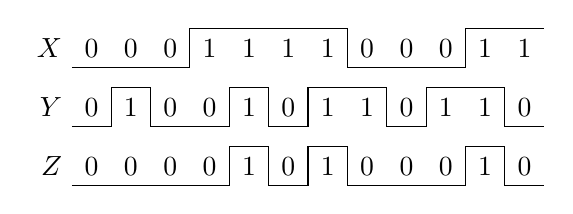
\begin{tikzpicture}
\pgfmathsetmacro{\kts}{0.5}
\pgfmathsetmacro{\kys}{0.5}
\pgfmathsetmacro{\kysep}{0.75}
\draw(0,0)node[above left]{$X$}--++(\kts,0)--++(\kts,0)--++(\kts,0)--++(0,\kys)--++(4*\kts,0)--++(0,-\kys)--++(3*\kts,0)--++(0,\kys)--++(2*\kts,0);
\draw(-\kts/2,0)
\foreach \n in {0,0,0,1,1,1,1,0,0,0,1,1}{++(\kts,0)node[above]{\n}};
\draw(0,-\kysep)node[above left]{$Y$}--++(\kts,0)--++(0,\kys)--++(\kts,0)--++(0,-\kys)--++(2*\kts,0)--++(0,\kys)--++(1*\kts,0)--++(0,-\kys)--++(1*\kts,0)--++(0,\kys)--++(2*\kts,0)--++(0,-\kys)--++(1*\kts,0)--++(0,\kys)--++(2*\kts,0)--++(0,-\kys)--++(1*\kts,0);
\draw(-\kts/2,-\kysep)
\foreach \n in {0,1,0,0,1,0,1,1,0,1,1,0}{++(\kts,0)node[above]{\n}};
\draw(0,-2*\kysep)node[above left]{$Z$}--++(4*\kts,0)--++(0,\kys)--++(\kts,0)--++(0,-\kys)--++(1*\kts,0)--++(0,\kys)--++(1*\kts,0)--++(0,-\kys)--++(3*\kts,0)--++(0,\kys)--++(1*\kts,0)--++(0,-\kys)--++(1*\kts,0);
\draw(-\kts/2,-2*\kysep)
\foreach \n in {0,0,0,0,1,0,1,0,0,0,1,0}{++(\kts,0)node[above]{\n}};
\end{tikzpicture}
\caption{ضرب گیٹ کی کارکردگی۔}
\label{شکل_بوولین_ضرب_جدول_دو_دخول}
\end{minipage}
\end{figure}

شکل  \حوالہ{شکل_بوولین_ضرب_جدول_دو_دخول}  میں دو مداخل   ضرب گیٹ کی کارکردگی  ترسیم  کی گئی ہے، جہاں \عددی{0} کو پست اور \عددی{1} کو بلند لکیر سے ظاہر کیا گیا ہے۔آپ دیکھ سکتے ہیں کہ مخارج صرف اور صرف اُس صورت بلند  ہوتا ہے جب ضرب گیٹ کے تمام مداخل بلند ہوں۔ ہم \عددی{0} کو پست اور \عددی{1} کو بلند بھی پکارتے ہیں۔ اس شکل میں  مداخل کو کسی خاص ترتیب سے  تبدیل نہیں  کیا گیا۔


ضرب گیٹ کو شکل \حوالہ{شکل_بوولین_گیٹ_بطور_سوئچ} میں بطور  عددی گیٹ یا عددی سوئچ  دکھایا گیا ہے جہاں  ایک داخلی پنیا  کو قابو پنیا  کا نام دیا گیا ہے جبکہ دوسرے کو   (اب بھی)  مداخل کہا گیا ہے۔ضرب گیٹ کے جدول سے واضح ہے کہ جب تک قابو پنیا  \عددی{0} ہو،   خارجی پنیا   \عددی{0}  رہتا ہے۔اس صورت میں   مداخل  پر موجود مواد، خارجی پنیا تک نہیں پہنچ سکتا،  یعنی   اس   پر \عددی{0} یا \عددی{1}  کا مخارج پر کوئی اثر نہیں ہوتا؛  ہم کہتے  ہیں قابو پنیا نے ضرب گیٹ کو معذور   کر دیا ۔اس کے برعکس اگر قابو پنیا  \عددی{1} ہو تب خارجی پنیا پر وہی کچھ ہوگا جو مداخل پر ہو گا؛ ہم کہتے  ہیں  ضرب گیٹ مجاز   کر دیا گیا ہے۔قابو پنیا پر ایک یا صفر  سے داخلی اشارہ  (مواد) کو خارجی پنیا تک پہنچنا،  ممکن یا ناممکن بنایا جا سکتا ہے۔یوں یہ ایک دروازے کی طرح کام کرتا ہے، جس   کی بنا   پر  یہ  گیٹ  کہلاتا ہے۔قابو پنیا کو،  معذور اور مجاز بنانے والا پنیا بھی کہتے ہیں۔شکل  \حوالہ{شکل_بوولین_گیٹ_کارکردگی}  میں ضرب   گیٹ کی  کارکردگی دکھائی گئی ہے۔آپ دیکھ سکتے ہیں کہ  صرف مجاز صورت میں مواد مخارج تک پہنچ پاتا ہے؛ معذور صورت میں مخارج ہمیشہ پست رہے گا۔

\begin{figure}
\centering
\begin{tikzpicture}
\draw(0,-2)node[above right]{مداخل}--++(2,0)--++(0.5,0.5)coordinate[pos=0.5](kk){}++(0,-0.5)--++(1.5,0)node[above left]{مخارج};
\draw[dashed](kk)--++(0,-1)--++(-1,0)node[left]{قابو};
\end{tikzpicture}\hfill
\begin{tikzpicture}
\draw(0,0)node[and port ,scale=1, number inputs=2](u1){};
\draw(0,0)node[and port](and1){};
\draw(u1.in 1)node[left]{مداخل};
\draw(u1.in 2)--++(0,-0.5)node[below]{قابو};
\draw(u1.out)node[right]{مخارج};
\end{tikzpicture}
\caption{ضرب گیٹ بطور  سوئچ یا ایک بِٹ گیٹ۔}
\label{شکل_بوولین_گیٹ_بطور_سوئچ}
\end{figure}
%
\begin{figure}
\centering
\begin{tikzpicture}
\pgfmathsetmacro{\kts}{0.5}
\pgfmathsetmacro{\kys}{0.5}
\pgfmathsetmacro{\kysep}{0.75}
\draw(0,0)node[above left]{قابو}--++(3*\kts,0)--++(0,\kys)--++(4*\kts,0)--++(0,-\kys)--++(5*\kts,0);
\draw(-\kts/2,0)
\foreach \n in {0,0,0,1,1,1,1,0,0,0,0,0}{++(\kts,0)node[above]{\n}};
\draw(0,-\kysep)node[above left]{مداخل}--++(\kts,0)--++(0,\kys)--++(\kts,0)--++(0,-\kys)--++(2*\kts,0)--++(0,\kys)--++(1*\kts,0)--++(0,-\kys)--++(1*\kts,0)--++(0,\kys)--++(2*\kts,0)--++(0,-\kys)--++(1*\kts,0)--++(0,\kys)--++(2*\kts,0)--++(0,-\kys)--++(1*\kts,0);
\draw(-\kts/2,-\kysep)
\foreach \n in {0,1,0,0,1,0,1,1,0,1,1,0}{++(\kts,0)node[above]{\n}};
\draw(0,-2*\kysep)node[above left]{مخارج}--++(4*\kts,0)--++(0,\kys)--++(\kts,0)--++(0,-\kys)--++(1*\kts,0)--++(0,\kys)--++(1*\kts,0)--++(0,-\kys)--++(5*\kts,0);
\draw(-\kts/2,-2*\kysep)
\foreach \n in {0,0,0,0,1,0,1,0,0,0,0,0}{++(\kts,0)node[above]{\n}};
\draw(1.5*\kts,0.75)node[]{معذور};
\draw(5*\kts,0.75)node[]{مجاز};
\draw(9.5*\kts,0.75)node[]{معذور};
\end{tikzpicture}
\caption{ضرب گیٹ کی کارکردگی۔}
\label{شکل_بوولین_گیٹ_کارکردگی}
\end{figure}


\جزوحصہ{جمع گیٹ}
منطقی جمع  (بوولین جمع)  تفاعل کو جمع گیٹ  سے عملی جامع پہنایا جاتا ہے۔  دو مداخل جمع گیٹ  شکل  \حوالہ{شکل_بوولین_ضرب_دو_متغیر_گیٹ}  میں دکھایا گیا ہے۔ یہ گیٹ،  جمع  تفاعل کے جدول  کو مطمئن کرتا ہے۔

\begin{figure}
\centering
\begin{minipage}[b]{0.40\textwidth}
\centering
\begin{tikzpicture}
\draw(0,0)node[or port ,scale=1, number inputs=2](u1){};
\draw(u1.in 1)node[left]{$X$}node[xshift=-0.25cm, yshift=0.75cm]{مداخل};
\draw(u1.in 2)node[left]{$Y$};
\draw(u1.out)node[right]{$Z$}node[xshift=0.25cm,yshift=1cm]{مخارج};
\end{tikzpicture}
\caption{دو مداخل جمع   گیٹ۔}
\label{شکل_بوولین_ضرب_دو_متغیر_گیٹ}
\end{minipage}\hfill
\begin{minipage}[b]{0.55\textwidth}
\centering
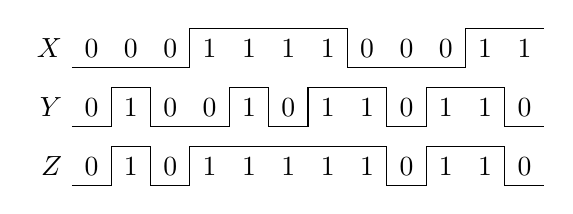
\begin{tikzpicture}
\pgfmathsetmacro{\kts}{0.5}
\pgfmathsetmacro{\kys}{0.5}
\pgfmathsetmacro{\kysep}{0.75}
\draw(0,0)node[above left]{$X$}--++(\kts,0)--++(\kts,0)--++(\kts,0)--++(0,\kys)--++(4*\kts,0)--++(0,-\kys)--++(3*\kts,0)--++(0,\kys)--++(2*\kts,0);
\draw(-\kts/2,0)
\foreach \n in {0,0,0,1,1,1,1,0,0,0,1,1}{++(\kts,0)node[above]{\n}};
\draw(0,-\kysep)node[above left]{$Y$}--++(\kts,0)--++(0,\kys)--++(\kts,0)--++(0,-\kys)--++(2*\kts,0)--++(0,\kys)--++(1*\kts,0)--++(0,-\kys)--++(1*\kts,0)--++(0,\kys)--++(2*\kts,0)--++(0,-\kys)--++(1*\kts,0)--++(0,\kys)--++(2*\kts,0)--++(0,-\kys)--++(1*\kts,0);
\draw(-\kts/2,-\kysep)
\foreach \n in {0,1,0,0,1,0,1,1,0,1,1,0}{++(\kts,0)node[above]{\n}};
\draw(0,-2*\kysep)node[above left]{$Z$}--++(1*\kts,0)--++(0,\kys)--++(\kts,0)--++(0,-\kys)--++(1*\kts,0)--++(0,\kys)--++(5*\kts,0)--++(0,-\kys)--++(1*\kts,0)--++(0,\kys)--++(2*\kts,0)--++(0,-\kys)--++(1*\kts,0);
\draw(-\kts/2,-2*\kysep)
\foreach \n in {0,1,0,1,1,1,1,1,0,1,1,0}{++(\kts,0)node[above]{\n}};
\end{tikzpicture}
\caption{جمع گیٹ کی کارکردگی۔}
\label{شکل_بوولین_جمع_جدول_دو_دخول}
\end{minipage}
\end{figure}

جمع گیٹ کی کارکردگی شکل  \حوالہ{شکل_بوولین_جمع_جدول_دو_دخول}  میں ترسیم کی  گئی ہے۔آپ دیکھ سکتے ہیں، جمع گیٹ کا مخارج اُس صورت  بلند ہوگا  جب کوئی   مداخل  بلند ہو۔

جمع گیٹ میں اگر ایک  پنیا  کو قابو  پنیا  سمجھا جائے تو پست  قابو،  گیٹ کو مجاز   بنا کر ،   داخلی مواد کو مخارج تک پہنچنے کی اجازت دیتا ہے،  جبکہ بلند قابو کی صورت میں مخارج لازماً بلند رہتا ہے۔

\جزوحصہ{نفی گیٹ}
نفی  تفاعل کو نفی گیٹ سے  عملی جامع پہنایا  جاتا ہے،  جس کی علامت شکل \حوالہ{شکل_بوولین_نفی_گیٹ}  میں دکھائی گئی ہے، اور جو  مواد کو مخارج تک پہنچنے سے    روک نہ  پانے کے  باوجود   (نفی) \قول{ گیٹ} کہلاتا ہے۔ اس کی کارکردگی شکل  \حوالہ{شکل_بوولین_نفی_کارکردگی}  میں ترسیم کی  گئی ہے۔آپ دیکھ سکتے ہیں،  نفی گیٹ کا مخارج اس کے مداخل کا اُلٹ  ہو گا۔ یہ گیٹ، نفی تفاعل کے جدول کو مطمئن کرتا ہے۔

\begin{figure}
\centering
\begin{minipage}[b]{0.4\textwidth}
\centering
\begin{tikzpicture}
\draw(0,0)node[not port ,scale=1, number inputs=1](u1){};
\draw(u1.in)node[left]{مداخل};
\draw(u1.out)node[right]{مخارج};
\end{tikzpicture}
\caption{نفی گیٹ}
\label{شکل_بوولین_نفی_گیٹ}
\end{minipage}\hfill
\begin{minipage}[b]{0.6\textwidth}
\centering
\begin{tikzpicture}
\pgfmathsetmacro{\kts}{0.5}
\pgfmathsetmacro{\kys}{0.5}
\pgfmathsetmacro{\kysep}{0.5}
\draw(0,0)node[above left]{مداخل}--++(2*\kts,0)--++(0,\kys)--++(1*\kts,0)--++(0,-\kys)--++(1*\kts,0)--++(0,\kys)--++(3*\kts,0)--++(0,-\kys)--++(2*\kys,0)--++(0,\kys)--++(\kts,0)--++(0,-\kys)--++(\kts,0)--++(0,\kys)--++(\kts,0);
\draw(-\kts/2,0)
\foreach \n in {0,0,1,0,1,1,1,0,0,1,0,1}{++(\kts,0)node[above]{\n}};
\draw(0,-\kysep)node[below left]{مخارج}--++(2*\kts,0)--++(0,-\kys)--++(1*\kts,0)--++(0,\kys)--++(1*\kts,0)--++(0,-\kys)--++(3*\kts,0)--++(0,\kys)--++(2*\kys,0)--++(0,-\kys)--++(\kts,0)--++(0,\kys)--++(\kts,0)--++(0,-\kys)--++(\kts,0);
\draw(-\kts/2,-\kysep-\kys)
\foreach \n in {1,1,0,1,0,0,0,1,1,0,1,0}{++(\kts,0)node[above]{\n}};
\end{tikzpicture}
\caption{نفی گیٹ کی کارکردگی۔}
\label{شکل_بوولین_نفی_کارکردگی}
\end{minipage}
\end{figure}

نفی تفاعل ایک  آزاد اور ایک  تابع متغیر رکھتا ہے، لہٰذا  نفی گیٹ کا ایک  مداخل اور ایک  مخارج ہو گا۔

\جزوحصہ{متعدد  مداخل گیٹ}
 ضرب گیٹ اور جمع گیٹ کے   متعدد  مداخل      ہو سکتے ہیں  (تاہم،  ان کا مخارج  ایک  ہو گا)۔  شکل  \حوالہ{شکل_بوولین_تین_ضرب_گیٹ}  میں تین مداخل ضرب گیٹ اور جدول،  اور شکل  \حوالہ{شکل_بوولین_تین_جمع} میں تین مداخل  جمع گیٹ اور جدول  دکھائے گئے ہیں، جہاں \عددی{A}، \عددی{B}، اور \عددی{C} مداخل جبکہ \عددی{Z} مخارج ہے۔ ضرب گیٹ کا مخارج اس  صورت بلند ہو گا جب  تمام مداخل بلند ہوں، جبکہ جمع گیٹ کا مخارج اس صورت بلند ہو گا جب کوئی بھی مداخل بلند ہو۔
 
\begin{figure}
\centering
\begin{minipage}{0.45\textwidth}
\centering
\begin{tikzpicture}
\draw(0,0)node[and port ,scale=1, number inputs=3](u1){};
\end{tikzpicture}%
\begin{otherlanguage}{english}
\begin{tabular}{CCC|C}
\toprule
A&B&C&Z\\
\midrule
0&0&0&0\\
0&0&1&0\\
0&1&0&0\\
0&1&1&0\\
1&0&0&0\\
1&0&1&0\\
1&1&0&0\\
1&1&1&1\\
\bottomrule
\end{tabular}
\end{otherlanguage} 
\caption{تین مداخل ضرب گیٹ۔}
\label{شکل_بوولین_تین_ضرب_گیٹ}
\end{minipage}\hfill
\begin{minipage}{0.45\textwidth}
\centering
\begin{tikzpicture}%
\draw(0,0)node[or port ,scale=1, number inputs=3](u1){};
\end{tikzpicture}
\begin{otherlanguage}{english}
\begin{tabular}{CCC|C}
\toprule
A&B&C&Z\\
\midrule
0&0&0&0\\
0&0&1&1\\
0&1&0&1\\
0&1&1&1\\
1&0&0&1\\
1&0&1&1\\
1&1&0&1\\
1&1&1&1\\
\bottomrule
\end{tabular}
\end{otherlanguage}
\caption{تین مداخل جمع گیٹ۔}
\label{شکل_بوولین_تین_جمع}
\end{minipage}
\end{figure}


شکل \حوالہ{شکل_بوولین_دو_ضرب_سے_تین} میں دو  ضرب گیٹ   یوں جوڑے گئے ہیں کہ ایک کا مخارج دوسرے کے مداخل سے جڑا ہے۔ساتھ ہی اس دور کا بوولین جدول دیا گیا ہے۔ پہلے جدول استعمال کیے بغیر اس دور کو سمجھنے کی کوشش کرتے ہیں۔ مخارج \عددی{Z}  اس صورت  بلند ہو گا جب دائیں گیٹ کے   مداخل  \عددی{C} اور \عددی{D} دونوں بلند ہوں لیکن \عددی{D} بلند ہونے کے لئے ضروری ہے کہ بائیں گیٹ کے مداخل  \عددی{A} اور \عددی{B} دونوں بلند ہوں۔ یوں  \عددی{A}، \عددی{B} اور \عددی{C} بلند ہونے کی صورت میں مخارج \عددی{Z} بلند ہو گا؛ یہی تین مداخل ضرب گیٹ کی خاصیت ہے۔


آئیں اب جدول کو  سمجھتے ہیں۔ تین مداخل \عددی{ABC} کے خانوں کو تین ہندسوں کے ثنائی اعداد  \عددی{000} تا \عددی{111} سے  پُر کریں۔ اس کے بعد بائیں ضرب گیٹ کے مخارج  \عددی{D} کے خانے پُر کریں۔ یاد رہے   کہ یہ صرف \عددی{A} اور \عددی{B} پر منحصر ہے اور صرف اس صورت بلند ہو گا جب یہ دونوں بلند ہوں، جو آخری دو صفوں میں ہو گا۔ اس کے بعد دائیں ضرب گیٹ کے مخارج \عددی{Z} کے خانے پُر کریں۔ یہ صرف \عددی{C} اور \عددی{D} پر منحصر ہے، اور بلند صرف اس صورت ہو گا جب یہ دونوں بلند ہوں۔

ان نتائج کا جدول \حوالہ{شکل_بوولین_تین_ضرب_گیٹ} میں پیش تین مداخل ضرب گیٹ کے  جدول کے ساتھ کریں۔آپ دیکھ سکتے ہیں کہ شکل \حوالہ{شکل_بوولین_دو_ضرب_سے_تین} میں دونوں ضرب گیٹ مل کر  تین مداخل  ضرب گیٹ کا کردار ادا کرتے ہیں۔ یوں دو داخلی ضرب گیٹوں کی مدد سے زیادہ مداخل کا ضرب گیٹ حاصل کیا جا سکتا ہے۔

 شکل  \حوالہ{شکل_بوولین_دو_جمع_سے_تین}  میں دو  مداخل جمع  گیٹوں  سے  تین  مداخل  جمع گیٹ کا حصول دکھایا گیا ہے۔  یہاں \عددی{Z} صرف اس صورت پست ہو گا جب دائیں گیٹ  کے دونوں مداخل، \عددی{C} اور \عددی{D}،  پست ہوں لیکن \عددی{D} صرف اس صورت پست ہو سکتا ہے جب بائیں گیٹ کے  مداخل، \عددی{A} اور \عددی{B}، پست ہوں۔ یوں \عددی{Z} صرف اس صورت پست ہو گا جب \عددی{A}، \عددی{B}، اور \عددی{C} پست ہوں، جو تین  مداخل جمع گیٹ کی  خاصیت ہے۔

\begin{figure}
\centering
\begin{otherlanguage}{english}
\begin{tikzpicture}
\draw(0,0)node[and port ,scale=1, number inputs=2](u1){};
\draw(2,-1)node[and port ,scale=1, number inputs=2](u2){};
\draw(u1.in 1)--++(-0.5,0)node[left]{A} (u1.in 2)--++(-0.5,0)node[left]{B} (u1.out)node[above]{D}-| (u2.in 1) (u2.in 2)--++(-2.5,0)node[left]{C} (u2.out)node[right]{Z};
\end{tikzpicture}\quad \quad 
\begin{tikzpicture}
\draw(0,0)node[]{
\begin{tabular}{CCC|C|C}
\toprule
A&B&C&D&Z\\
\midrule
0&0&0&0&0\\
0&0&1&0&0\\
0&1&0&0&0\\
0&1&1&0&0\\
1&0&0&0&0\\
1&0&1&0&0\\
1&1&0&1&0\\
1&1&1&1&1\\
\bottomrule
\end{tabular}
};
\end{tikzpicture}
\end{otherlanguage}
\caption{دو مداخل ضرب گیٹ سے تین مداخل ضرب گیٹ کا حصول۔}
\label{شکل_بوولین_دو_ضرب_سے_تین}
\end{figure}
%
\begin{figure}
\centering
\begin{otherlanguage}{english}
\begin{tikzpicture}
\draw(0,0)node[or port ,scale=1, number inputs=2](u1){}; 
\draw(2,-1)node[or port ,scale=1, number inputs=2](u2){};
\draw(u1.in 1)--++(-0.5,0)node[left]{A} (u1.in 2)--++(-0.5,0)node[left]{B} (u1.out)node[above]{D}-| (u2.in 1) (u2.in 2)--++(-2.5,0)node[left]{C} (u2.out)node[right]{Z};
\end{tikzpicture}\quad \quad %
\begin{tikzpicture}
\draw(0,0)node[]{
\begin{tabular}{CCC|C|C}
\toprule
A&B&C&D&Z\\
\midrule
0&0&0&0&0\\
0&0&1&0&1\\
0&1&0&1&1\\
0&1&1&1&1\\
1&0&0&1&1\\
1&0&1&1&1\\
1&1&0&1&1\\
1&1&1&1&1\\
\bottomrule
\end{tabular}
};
\end{tikzpicture}
\end{otherlanguage}
\caption{دو مداخل جمع گیٹ سے تین مداخل جمع گیٹ کا حصول۔}
\label{شکل_بوولین_دو_جمع_سے_تین}
\end{figure}
%

\begin{figure}
\centering
\begin{subfigure}{1\textwidth}
\centering
\begin{tikzpicture}
\pgfmathsetmacro{\kxs}{3}
\pgfmathsetmacro{\kys}{1.25}
\draw(0,0)node[or port ,scale=1, number inputs=2](u1){u1} (0,-\kys)node[or port ,scale=1, number inputs=2](u2){u2} (\kxs,-\kys/2)node[or port ,scale=1, number inputs=2](u3){u3};
\draw(u1.in 1)node[left]{$A$} (u1.in 2)node[left]{$B$} (u2.in 1)node[left]{$C$} (u2.in 2)node[left]{$D$};
\draw(u1.out)node[above right]{$A+B$}-|(u3.in 1) (u2.out)node[below right]{$C+D$}-|(u3.in 2) (u3.out)node[right]{$(A+B)+(C+D)$};
\end{tikzpicture}
\caption{}
\end{subfigure}
\begin{subfigure}{1\textwidth}
\centering
\begin{tikzpicture}
\pgfmathsetmacro{\kxs}{3}
\pgfmathsetmacro{\kys}{1.25}
\draw(0,0)node[or port ,scale=1, number inputs=2](u4){u4} (0,-\kys)node[or port ,scale=1, number inputs=2](u5){u5} (\kxs,-\kys/2)node[and port ,scale=1, number inputs=2](u6){u6};
\draw(u4.in 1)node[left]{$A$} (u4.in 2)node[left]{$B$} (u5.in 1)node[left]{$C$} (u5.in 2)node[left]{$D$};
\draw(u4.out)node[above right]{$A+B$}-|(u6.in 1) (u5.out)node[below right]{$C+D$}-|(u6.in 2) (u6.out)node[right]{$(A+B)(C+D)$};
\end{tikzpicture}
\caption{}
\end{subfigure}
\caption{جمع اور ضرب گیٹ کے ادوار۔}
\label{شکل_بوولین_جمع_ضرب_ادوار}
\end{figure}
 جمع گیٹ اور ضرب گیٹ   پر مبنی، شکل  \حوالہ{شکل_بوولین_جمع_ضرب_ادوار}میں دکھائے  گئے    ادوار کو   مثال بنا کر،   عددی  ادوار   حل کرنا سیکھتے ہیں۔
 
 شکل  \حوالہ{شکل_بوولین_جمع_ضرب_ادوار}-الف سے آغاز کرتے ہیں جہاں  گیٹوں کو \عددی{u1}، \عددی{u2}، اور \عددی{u3} کے نام دیے گئے ہیں۔  جمع گیٹ \عددی{u1} اور \عددی{u2}  کے خارجی پنیے،           جمع گیٹ \عددی{u3}  کے داخلی  پنیوں    سے جڑے    ہیں۔ چونکہ \عددی{u1} کا مخارج \عددی{A+B} اور \عددی{u2} کا مخارج \عددی{C+D} دیگا، لہٰذا \عددی{u3} کا مخارج \عددی{(A+B)+(C+D)} یعنی \عددی{A+B+C+D} دیگا۔  


آئیں ا ب  شکل  \حوالہ{شکل_بوولین_جمع_ضرب_ادوار}-ب حل  ہیں۔ یہاں  \عددی{u4} اور \عددی{u5} کے مخارج بالترتیب \عددی{A+B} اور \عددی{C+D} دیں گے۔ چونکہ \عددی{u6} ضرب گیٹ ہے،   لہٰذا اس کا مخارج \عددی{(A+B)(C+D)} دیگا۔
\begin{figure}
\centering
\begin{subfigure}{1\textwidth}
\centering
\begin{tikzpicture}
\pgfmathsetmacro{\kxs}{3}
\pgfmathsetmacro{\kys}{1}
\draw(0,0)node[or port ,scale=1, number inputs=2](u1){u1} (0,-1.5*\kys)node[or port ,scale=1, number inputs=2](u2){u2} (\kxs,-\kys/2)node[and port ,scale=1, number inputs=2](u3){u3} (\kxs,-2*\kys)node[not port ,scale=1, number inputs=1, label={[xshift=-0.5em,yshift=-0.5em]u4}](u4){};
\draw(u1.in 1)node[left]{$A$} (u1.in 2)node[left]{$B$} (u2.in 1)node[left]{$C$} (u2.in 2)node[left]{$D$};
\draw(u1.out)node[above right]{$A+B$}-|(u3.in 1) (u2.out)node[below right]{$C+D$}-|coordinate(ktt)(u3.in 2) (u3.out)node[right]{$(A+B)(C+D)$};
\draw(ktt)|-(u4.in)  (u4.out)node[right]{$\overline{C+D}$};
\end{tikzpicture}
\caption{}
\end{subfigure}
\begin{subfigure}{1\textwidth}
\centering
\begin{tikzpicture}%[circuit logic US,minimum height=1cm] 
\pgfmathsetmacro{\kxs}{3}
\pgfmathsetmacro{\kys}{1.5}
\draw (0,0) node[or port ,scale=1, number inputs=3](u5){u5};
\draw (0,-\kys) node[or port ,scale=1, number inputs=2](u6){u6};
\draw (1*\kxs,-\kys/2) node[and port ,scale=1, number inputs=2](u7){u7};
\draw(u5.in 1)node[left]{$E$} (u5.in 2)node[left]{$F$} (u5.in 3)node[left]{$G$} 
(u6.in 1)node[left]{$H$} (u6.in 2)node[left]{$I$} (u7.out)node[right]{$(E+F+G)(H+I)$};
\draw(u5.out)node[above right]{$E+F+G$}-|(u7.in 1);
\draw(u6.out)node[below right]{$H+I$}-|(u7.in 2);
\end{tikzpicture}
\caption{}
\end{subfigure}
\caption{گیٹوں کا دوسرا دور۔}
\label{شکل_بوولین_جمع_ضرب_دوسرا_ادوار}
\end{figure}

شکل \حوالہ{شکل_بوولین_جمع_ضرب_دوسرا_ادوار}-الف  میں \عددی{u2} کا مخارج \عددی{u3} کے مداخل اور \عددی{u4} کے مداخل کے ساتھ  جڑا ہے۔ گیٹ \عددی{u1} اور \عددی{u2} کے مخارج بالترتیب \عددی{A+B} اور \عددی{C+D} ہیں۔ گیٹ \عددی{u3} کا مخارج \عددی{(A+B)(C+D)} اور \عددی{u4} کا مخارج \عددی{\overline{C+D}} ہو گا۔

 آپ  شکل \حوالہ{شکل_بوولین_جمع_ضرب_دوسرا_ادوار}-ب  کا حل،  شکل کو دیکھ کر   سمجھ سکتے ہیں۔ 


\جزوحصہ{ضرب متمم  گیٹ اور جمع متمم گیٹ}
شکل  \حوالہ{شکل_بوولین_ضرب_متمم}-الف  میں تین مداخل ضرب گیٹ کا مخارج \عددی{ABC} ہو گا، جو نفی گیٹ کا مداخل ہے، لہٰذا نفی گیٹ کا مخارج \عددی{Z=\overline{ABC}} ہوگا۔ ضرب گیٹ کے مخارج کا متمم اتنی اہمیت رکھتا ہے کہ اس کے لئے علیحدہ گیٹ  بنایا گیا ہے، جسے ضرب متمم گیٹ (یا ضد ضرب گیٹ)  کہتے ہیں اور جو شکل-ب میں  (تین مداخل کے لئے)   دکھایا گیا ہے۔ ضرب گیٹ کے جدول کا متمم لینے سے ضرب متمم گیٹ  کا جدول حاصل ہو گا   جو اسی شکل   میں پیش کیا گیا ہے۔

 دو مداخل ضرب متمم گیٹ کی مساوات درج ذیل ہو گی، جہاں \عددی{X} اور \عددی{Y} مداخل جبکہ \عددی{Z} مخارج ہے۔
\begin{align}
Z&=\overline{XY}=\overline{X}+\overline{Y}&\text{\RL{\small{(ضرب متمم)}}}
\end{align}


\begin{figure}
\centering
\begin{minipage}{0.8\textwidth}
\centering
\begin{subfigure}{1\textwidth}
\centering
\begin{tikzpicture}%[circuit logic US,minimum height=1cm] 
\pgfmathsetmacro{\kxs}{1.75}
\pgfmathsetmacro{\kys}{1.5}
\draw(0,0)node[and port ,scale=1, number inputs=3](u1){} (\kxs,0) node[not port, scale=1, number inputs=1](u2){};
\draw(u1.in 1)node[left]{$A$} (u1.in 2)node[left]{$B$} (u1.in 3)node[left]{$C$}
 (u2.out)node[above right]{$Z=\overline{ABC}$};
\draw(u1.out)node[above right,xshift=-0.5em]{$ABC$}--(u2.in);
\end{tikzpicture}
\caption{}
\end{subfigure}
\begin{subfigure}{1\textwidth}
\centering
\begin{otherlanguage}{english}
\begin{tikzpicture}
\pgfmathsetmacro{\kxs}{3}
\pgfmathsetmacro{\kys}{1}
\draw(0,0)node[nand port ,scale=1, number inputs=3](u1){};
\draw(u1.in 1)node[left]{$A$} (u1.in 2)node[left]{$B$} (u1.in 3)node[left]{$C$}
 (u1.out)node[right]{$Z=\overline{ABC}$};
\end{tikzpicture}
\end{otherlanguage}
\caption{}
\end{subfigure}
\end{minipage}\hfill
\begin{minipage}{0.2\textwidth}
\centering
\begin{otherlanguage}{english}
\begin{tabular}{CCC|C}
\toprule
A&B&C&Z\\
\midrule
0&0&0&1\\
0&0&1&1\\
0&1&0&1\\
0&1&1&1\\
1&0&0&1\\
1&0&1&1\\
1&1&0&1\\
1&1&1&0\\
\bottomrule
\end{tabular}
\end{otherlanguage}
\end{minipage}
\caption{ضرب متمم گیٹ یا ضد ضرب گیٹ۔}
\label{شکل_بوولین_ضرب_متمم}
\end{figure}
%
\begin{figure}
\centering
\begin{minipage}{0.8\textwidth}
\centering
\begin{subfigure}{1\textwidth}
\centering
\begin{tikzpicture}%[circuit logic US,minimum height=1cm] 
\pgfmathsetmacro{\kxs}{2}
\pgfmathsetmacro{\kys}{1.5}
\draw(0,0)node[or port ,scale=1, number inputs=3](u1){} (\kxs,0) node[not port, scale=1, number inputs=1](u2){};
\draw(u1.in 1)node[left]{$A$} (u1.in 2)node[left]{$B$} (u1.in 3)node[left]{$C$}
 (u2.out)node[above right,font=\small,xshift=-0.5em]{$Z=\overline{A+B+C}$};
\draw(u1.out)node[above right,xshift=-0.5em,font=\small,xshift=-0.5em]{$A+B+C$}--(u2.in);
\end{tikzpicture}
\caption{}
\end{subfigure}
\begin{subfigure}{1\textwidth}
\centering
\begin{tikzpicture}
\pgfmathsetmacro{\kxs}{3}
\pgfmathsetmacro{\kys}{1}
\draw(0,0)node[nor port ,scale=1, number inputs=3](u1){};
\draw(u1.in 1)node[left]{$A$} (u1.in 2)node[left]{$B$} (u1.in 3)node[left]{$C$}
 (u1.out)node[right]{$Z=\overline{A+B+C}$};
\end{tikzpicture}
\caption{}
\end{subfigure}
\end{minipage}\hfill
\begin{minipage}{0.2\textwidth}
\centering
\begin{otherlanguage}{english}
\begin{tabular}{CCC|C}
\toprule
A&B&C&Z\\
\midrule
0&0&0&1\\
0&0&1&0\\
0&1&0&0\\
0&1&1&0\\
1&0&0&0\\
1&0&1&0\\
1&1&0&0\\
1&1&1&0\\
\bottomrule
\end{tabular}
\end{otherlanguage}
\end{minipage}
\caption{جمع متمم گیٹ یا ضد جمع گیٹ۔}
\label{شکل_بوولین_جمع_متمم}
\end{figure}


شکل  \حوالہ{شکل_بوولین_جمع_متمم}-الف  میں تین مداخل  جمع  گیٹ کا مخارج \عددی{A+B+C} ہو گا، جو نفی گیٹ کا مداخل ہے، لہٰذا نفی گیٹ کا مخارج \عددی{Z=\overline{A+B+C}} ہوگا۔ جمع  گیٹ کے مخارج کا متمم اتنی اہمیت رکھتا ہے کہ اس کے لئے علیحدہ گیٹ  بنایا گیا ہے، جسے جمع  متمم گیٹ (یا ضد جمع گیٹ) کہتے ہیں اور جو شکل-ب میں (تین مداخل کے لئے)  دکھایا گیا ہے۔  جمع  گیٹ کے جدول کا متمم لینے سے جمع متمم گیٹ  کا جدول حاصل ہو گا جو اسی شکل  میں  پیش کیا گیا ہے۔

 دو مداخل جمع متمم گیٹ کی مساوات درج ذیل ہو گی، جہاں \عددی{X} اور \عددی{Y} مداخل جبکہ \عددی{Z} مخارج ہے۔
\begin{align}
Z&=\overline{X+Y}=\overline{X}\cdot\overline{Y}&\text{\RL{\small{(جمع متمم)}}}
\end{align}



\begin{figure}
\centering
\begin{tikzpicture}
\draw(0,0)node[nor port, scale=1, number inputs=2](u1){};
\draw(u1.in 1)--(u1.in 2)coordinate[pos=0.5](kk);
\draw(kk)--++(-0.5,0)node[left]{$X$};
\draw(u1.out)node[right]{$Z=\overline{X+ X}=\overline{X}$};
\end{tikzpicture}\quad\quad\quad
\begin{tikzpicture}
\draw(0,0)node[nand port, scale=1, number inputs=2](u1){};
\draw(u1.in 1)--(u1.in 2)coordinate[pos=0.5](kk);
\draw(kk)--++(-0.5,0)node[left]{$X$};
\draw(u1.out)node[right]{$Z=\overline{X\cdot X}=\overline{X}$};
\end{tikzpicture}
\caption{ضرب متمم اور جمع متمم گیٹ سے نفی گیٹ کا حصول۔}
\label{شکل_بوولین_نفی_حصول}
\end{figure}

شکل  \حوالہ{شکل_بوولین_نفی_حصول} میں ضرب متمم اور جمع متمم گیٹ سے نفی گیٹ کا حصول دکھایا گیا ہے۔ ضرب متمم کے دونوں مداخل کو آپس میں جوڑا گیا ہے، لہٰذا دونوں مداخل  پر \عددی{X} ہو گا۔یوں مخارج \عددی{Z=\overline{X\cdot X}} یعنی \عددی{Z=\overline{X}}  ہو گا؛ یہاں اس حقیقت کو استعمال کیا گیا ہے کہ اگر \عددی{X=0} ہو تب \عددی{X\cdot X} بھی \عددی{0} ہو گا، اور اگر \عددی{X=1} ہو تب \عددی{X\cdot X} بھی \عددی{1} ہو گا، لہٰذا \عددی{X\cdot X=X} لکھا جا سکتا ہے۔  نفی گیٹ کا مخارج بھی یہی (\عددی{Z=\overline{X}})    دیگا،  لہٰذا ضرب گیٹ کے دونوں مداخل آپس میں جوڑنے سے نفی گیٹ کی کارکردگی حاصل ہو گی۔ اسی طرح (تسلی کر لیں کہ)  جمع گیٹ کے مداخل آپس میں جوڑنے سے بھی نفی گیٹ حاصل ہو گا۔

 شکل \حوالہ{شکل_بوولین_متمم_سے_جمع_ضرب}-الف  میں تین  جمع متمم  گیٹ یوں جوڑے گئے ہیں کہ \عددی{Z=XY} حاصل ہو،  جو   ضرب گیٹ کی کارکردگی ہے۔یوں جمع متمم گیٹوں سے ضرب گیٹ حاصل ہو گا۔

 شکل \حوالہ{شکل_بوولین_متمم_سے_جمع_ضرب}-ب  میں  جمع گیٹ کا حصول دکھایا گیا ہے۔  اس کا مخارج \عددی{Z=X+Y} ہے۔
 
   شکل \حوالہ{شکل_بوولین_ضرب_متمم_سے_جمع_ضرب} میں ضرب متمم گیٹ سے (ا)  جمع  گیٹ  اور  (ب) ضرب  گیٹ کا حصول دکھایا گیا ہے۔ 


\begin{figure}
\centering
\begin{subfigure}{1\textwidth}
\centering
\begin{tikzpicture}
\pgfmathsetmacro{\kxs}{4}
\pgfmathsetmacro{\kys}{1.5}
\draw(0,0)node[nor port ,scale=1, number inputs=2](u1){};
\draw(0,-\kys)node[nor port ,scale=1, number inputs=2](u2){};
\draw(\kxs,-\kys/2)node[nor port ,scale=1, number inputs=2](u3){};
\draw(u1.in 1)--(u1.in 2)coordinate[pos=0.5](kXX) (kXX)--++(-0.5,0)node[left]{$X$};
\draw(u2.in 1)--(u2.in 2)coordinate[pos=0.5](kYY) (kYY)--++(-0.5,0)node[left]{$Y$};
\draw(u1.out)node[above]{$\overline{X}$}-|(u3.in 1);
\draw(u2.out)node[above]{$\overline{Y}$}-|(u3.in 2);
\draw(u3.out)node[right]{$Z=\overline{\overline{X}+\overline{Y}}=\overline{\overline{X}}\cdot\overline{\overline{Y}}=XY$};
\end{tikzpicture}
\caption{}
\end{subfigure}
\begin{subfigure}{1\textwidth}
\centering
\begin{tikzpicture}
\pgfmathsetmacro{\kxs}{4}
\pgfmathsetmacro{\kys}{1.5}
\draw(0,0)node[nor port ,scale=1, number inputs=2](u1){};
\draw(\kxs,0)node[nor port ,scale=1, number inputs=2](u2){};
\draw(u2.in 1)--(u2.in 2)coordinate[pos=0.5](kk);
\draw(u1.out)node[above right]{$\overline{X+Y}$}--(kk);
\draw(u2.out)node[right]{$Z=\overline{\overline{X+Y}}=X+Y$};
\draw(u1.in 1)node[left]{$X$} (u1.in 2)node[left]{$Y$};
\end{tikzpicture}
\caption{}
\end{subfigure}
\caption{جمع متمم سے (ا)  ضرب گیٹ  اور  (ب) جمع گیٹ کا حصول۔}
\label{شکل_بوولین_متمم_سے_جمع_ضرب}
\end{figure}
%
\begin{figure}
\centering
\begin{subfigure}{1\textwidth}
\centering
\begin{tikzpicture}
\pgfmathsetmacro{\kxs}{4}
\pgfmathsetmacro{\kys}{1.5}
\draw(0,0)node[nand port ,scale=1, number inputs=2](u1){};
\draw(0,-\kys)node[nand port ,scale=1, number inputs=2](u2){};
\draw(\kxs,-\kys/2)node[nand port ,scale=1, number inputs=2](u3){};
\draw(u1.in 1)--(u1.in 2)coordinate[pos=0.5](kXX) (kXX)--++(-0.5,0)node[left]{$X$};
\draw(u2.in 1)--(u2.in 2)coordinate[pos=0.5](kYY) (kYY)--++(-0.5,0)node[left]{$Y$};
\draw(u1.out)node[above]{$\overline{X}$}-|(u3.in 1);
\draw(u2.out)node[above]{$\overline{Y}$}-|(u3.in 2);
\draw(u3.out)node[right]{$Z=\overline{\overline{X}\cdot\overline{Y}}=\overline{\overline{X}}+\overline{\overline{Y}}=X+Y$};
\end{tikzpicture}
\caption{}
\end{subfigure}
\begin{subfigure}{1\textwidth}
\centering
\begin{tikzpicture}
\pgfmathsetmacro{\kxs}{4}
\pgfmathsetmacro{\kys}{1.5}
\draw(0,0)node[nand port ,scale=1, number inputs=2](u1){};
\draw(\kxs,0)node[nand port ,scale=1, number inputs=2](u2){};
\draw(u2.in 1)--(u2.in 2)coordinate[pos=0.5](kk);
\draw(u1.out)node[above right]{$\overline{X\cdot Y}$}--(kk);
\draw(u2.out)node[right]{$Z=\overline{\overline{X\cdot Y}}=XY$};
\draw(u1.in 1)node[left]{$X$} (u1.in 2)node[left]{$Y$};
\end{tikzpicture}
\caption{}
\end{subfigure}
\caption{ضرب متمم سے (ا)  جمع گیٹ  اور (ب)  ضرب گیٹ کا حصول۔}
\label{شکل_بوولین_ضرب_متمم_سے_جمع_ضرب}
\end{figure}


\جزوحصہ{بلا شرکت جمع گیٹ اور  بلا شرکت جمع متمم  گیٹ}
بلا شرکت جمع تفاعل کو بلا شرکت جمع گیٹ  سے حاصل کیا جاتا ہے جس کا جدول اور  علامت،    شکل  \حوالہ{شکل_بوولین_بلاشرکت_متمم}-الف  میں پیش   کیے گئے ہیں۔اسی طرح بلا شرکت  جمع متمم  (یا ضد بلا شرکت جمع)   تفاعل کو  بلا شرکت جمع متمم  گیٹ (یعنی ضد بلا شرکت جمع گیٹ)    کی مدد سے حاصل کیا جاتا ہے جس کا جدول اور علامت،      شکل-ب میں پیش کیے گئے ہیں۔

بلا شرکت جمع گیٹ کے  مخارج کے ساتھ نفی گیٹ منسلک کرنے سے بلا شرکت جمع متمم  گیٹ حاصل کیا جا سکتا ہے۔بلا شرکت جمع  گیٹ کی کارکردگی شکل \حوالہ{شکل_بوولین_بلاشرکت_کارکردگی} میں دکھائی گئی ہے، جہاں \عددی{X} اور \عددی{Y} مداخل جبکہ \عددی{Z} مخارج ہے۔
	
تین مداخل  بلا شرکت جمع گیٹ کا مخارج حاصل کرنے کے لئے  اس کے کسی دو مداخل کا بلا شرکت جمع حاصل کریں اور حاصل جواب کا تیسرے مداخل کے ساتھ بلا شرکت جمع  لیں۔ یہی      بلا شرکت جمع ہو گا۔متعدد مداخل  بلا شرکت جمع گیٹ کا مخارج اُس صورت بلند ہوگا  جب  بلند مداخل کی تعداد طاق ہو۔

 \begin{figure}
 \centering
 \begin{subfigure}{0.45\textwidth}
 \centering
 \begin{tikzpicture}
  \draw(0,0)node[xor port, scale=1, number inputs=2](){};
 \end{tikzpicture}%
 \begin{otherlanguage}{english}
\begin{tabular}{CCC|C}
\toprule
A&B&C&Z\\
\midrule
0&0&0&0\\
0&0&1&1\\
0&1&0&1\\
0&1&1&0\\
1&0&0&1\\
1&0&1&0\\
1&1&0&0\\
1&1&1&1\\
\bottomrule
\end{tabular}
\end{otherlanguage}
 \caption{}
 \end{subfigure}\hfill
  \begin{subfigure}{0.45\textwidth}
 \centering
 \begin{tikzpicture}
 \draw(0,0)node[xnor port, scale=1, number inputs=2](){};
 \end{tikzpicture}%
 \begin{otherlanguage}{english}
\begin{tabular}{CCC|C}
\toprule
A&B&C&Z\\
\midrule
0&0&0&1\\
0&0&1&0\\
0&1&0&0\\
0&1&1&1\\
1&0&0&0\\
1&0&1&1\\
1&1&0&1\\
1&1&1&0\\
\bottomrule
\end{tabular}
\end{otherlanguage}
 \caption{}
 \end{subfigure}
 \caption{(ا) بلا شرکت جمع  گیٹ اور  (ب) بلا شرکت جمع  متمم گیٹ۔}
 \label{شکل_بوولین_بلاشرکت_متمم}
 \end{figure}
%
\begin{figure}
\centering
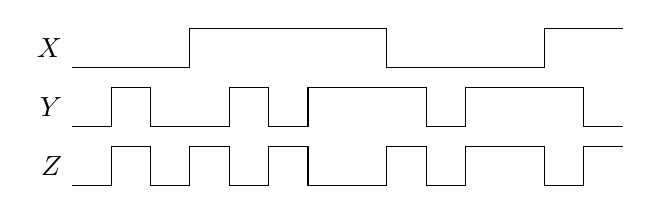
\begin{tikzpicture}
\pgfmathsetmacro{\kts}{0.5}
\pgfmathsetmacro{\kys}{0.5}
\pgfmathsetmacro{\kysep}{0.75}
\draw(0,0)node[above left]{$X$}--++(3*\kts,0)--++(0,\kys)--++(5*\kts,0)--++(0,-\kys)--++(4*\kts,0)--++(0,\kys)--++(2*\kts,0);
\draw(0,-\kysep)node[above left]{$Y$}--++(1*\kts,0)--++(0,\kys)--++(1*\kts,0)--++(0,-\kys)--++(2*\kts,0)--++(0,\kys)--++(\kts,0)
--++(0,-\kys)--++(\kts,0)--++(0,\kys)--++(3*\kts,0)--++(0,-\kys)--++(\kts,0)--++(0,\kys)--++(3*\kts,0)--++(0,-\kys)--++(\kts,0);
\draw(0,-2*\kysep)node[above left]{$Z$}--++(\kts,0)--++(0,\kys)--++(\kts,0)--++(0,-\kys)--++(\kts,0)--++(0,\kys)--++(\kts,0)--++(0,-\kys)--++(\kts,0)--++(0,\kys)--++(\kts,0)--++(0,-\kys)--++(2*\kts,0)--++(0,\kys)--++(\kts,0)--++(0,-\kys)--++(\kts,0)--++(0,\kys)--++(2*\kts,0)--++(0,-\kys)--++(\kts,0)--++(0,\kys)--++(\kts,0);
\end{tikzpicture}
\caption{بلا شرکت جمع گیٹ کی کارکردگی۔}
\label{شکل_بوولین_بلاشرکت_کارکردگی}
\end{figure}

آپ  سے گزارش  ہے کہ مذکورہ بالا تفاعلات اور گیٹوں کو اچھی طرح سمجھیں اور ذہن نشین کریں۔



\حصہ{گیٹوں کے  برقی خواص}  
گیٹ  (کا  مخارج)   اس صورت بلند تصور کیا جاتا ہے جب اس  ( کے مخارج پنیا) کا    خارجی دباو  ایک مخصوص قیمت  یا اس سے زیادہ  ہو۔یہ قیمت    بلند خارجی برقی دباو \عددی{V_{OH}}    کہلاتی ہے۔بلند صورت میں گیٹ  مخارج پنیے پر  ایک مخصوص قیمت  تک برقی رو خارج (مہیا)  کر سکتا ہے ، جو گیٹ کا  بلند خارجی برقی رو \عددی{I_{OH}}   کہلاتا ہے۔

گیٹ (کا مخارج)  اس صورت پست تصور کیا جاتا ہے جب اس (کے مخارج پنیا) کا خارجی دباو  ایک مخصوص قیمت  یا اس سے کم  ہو۔یہ  قیمت پست  خارجی برقی دباو \عددی{V_{OL}}   کہلاتی ہے۔پست   گیٹ،   مخارج پنیے پر  ایک مخصوص قیمت  تک برقی رو جذب   کر سکتا ہے ، جو گیٹ کا  پست خارجی    برقی رو   \عددی{I_{OL}} کہلاتا ہے۔

	
گیٹ ایک مخصوص  قیمت  اور اس سے زیادہ داخلی برقی دباو کو بلند تصور کرتا ہے۔اس برقی دباو کو بلند داخلی برقی دباو \عددی{V_{IH}}  کہتے ہیں۔گیٹ کے کسی ایک مداخل کو بلند کرنے کی خاطر درکار برقی رو کو بلند داخلی برقی رو   \عددی{I_{IH}} کہتے ہیں۔

گیٹ ایک مخصوص قیمت اور اس سے کم داخلی برقی دباو کو پست تصور کرتا ہے۔اس قیمت  کو پست داخلی برقی دباو   \عددی{V_{IL}} کہتے ہیں۔گیٹ کے کسی ایک مداخل کو پست کرنے کی خاطر درکار برقی رو کو پست داخلی برقی رو  \عددی{I_{IL}} کہتے ہیں۔
	
  گیٹوں کو  آپس میں برقی  تاروں سے   جوڑا جاتا ہے۔کبھی کبھار ان تاروں میں،  جائے استعمال پر پائے جانے  والے تغیر پذیر برقی و مقناطیسی میدان  کی وجہ سے،  غیر ضروری اور ناپسندیدہ   برقی دباو پیدا ہوتا ہے جسے  برقی شور  کہتے ہیں۔ایک گیٹ کے پست خارجی برقی دباو    کے ساتھ یہ  شور  جمع ہو کر اگلے گیٹ کے   پست داخلی برقی دباو   سے تجاوز کر سکتا ہے۔اسی طرح  برقی شور بلند خارجی برقی دباو سے نفی ہو کر بلند داخلی برقی دباو  سے  کم ہو سکتا ہے۔ان دونوں  صورتوں  میں اگلا گیٹ   غیر متوقع   نتائج دیگا۔

 بلند خارجی برقی دباو کی قیمت ،  بلند داخلی برقی دباو کی قیمت سے  زیادہ ہوتی ہے۔ان کے فرق کو بلند شور  گنجائش \عددی{V_{NH}}    کہتے ہیں (شکل \حوالہ{شکل_بوولین_گنجائش_شور} دیکھیں)۔
\begin{align}
V_{NH}=V_{OH}-V_{IH}
\end{align}
 پست خارجی برقی دباو کی قیمت، پست  داخلی برقی دباو  کی قیمت سے  کم ہوتی ہے۔ان کے فرق کو پست شور  گنجائش \عددی{V_{NL}}   کہتے ہیں۔
\begin{align}
V_{NL}=V_{IL}-V_{OL}
\end{align}


\begin{figure}
\centering
\begin{tikzpicture}
\pgfmathsetmacro{\kkx}{2}
\pgfmathsetmacro{\kky}{3}
\pgfmathsetmacro{\kkOL}{0.65}
\pgfmathsetmacro{\kkOH}{2.35}
\pgfmathsetmacro{\kTOL}{\kkOL/2}
\pgfmathsetmacro{\kTOH}{(\kky+\kkOH)/2}
\pgfmathsetmacro{\kkIL}{0.85}
\pgfmathsetmacro{\kkIH}{2}
\pgfmathsetmacro{\kTIL}{\kkIL/2}
\pgfmathsetmacro{\kTIH}{(\kky+\kkIH)/2}
\pgfmathsetmacro{\kkxsep}{4}
\draw(0,0)node[left]{$0$} rectangle ++(\kkx,\kky);
\draw(0,\kkOL)node[left]{$V_{OL}$}--++(\kkx,0);
\draw(0,\kkOH)node[left]{$V_{OH}$}--++(\kkx,0);
\draw(\kkxsep,0) rectangle ++(\kkx,\kky);
\draw(\kkxsep,\kkIL)--++(\kkx,0)node[right]{$V_{IL}$};
\draw(\kkxsep,\kkIH)--++(\kkx,0)node[right]{$V_{IH}$};
\draw[dashed] (\kkx,\kkOL)--++(1.5,0)coordinate[pos=0.75](kkL);
\draw[dashed] (\kkx,\kkOH)--++(1.5,0)coordinate[pos=0.6](kkH);
\draw[dashed] (\kkxsep,\kkIL)--++(-1.5,0);
\draw[dashed] (\kkxsep,\kkIH)--++(-1.5,0);
\draw[<-] (kkL)--++(0,-0.5)node[below]{$V_{NL}$};
\draw[<-]($(kkL)+(0,\kkIL-\kkOL)$)--++(0,0.25);
\draw[<-] (kkH)--++(0,0.5)node[above]{$V_{NH}$};
\draw[<-]($(kkH)+(0,\kkIH-\kkOH)$)--++(0,-0.25);
\draw(\kkx/2,\kTOL)node[]{\RL{خارجی پست}};
\draw(\kkx/2,\kTOH)node[]{\RL{خارجی بلند}};
\draw(\kkxsep+\kkx/2,\kTIL)node[]{\RL{داخلی  پست}};
\draw(\kkxsep+\kkx/2,\kTIH)node[]{\RL{داخلی  بلند}};
\draw(0,\kky)node[left]{$V_{DD}$};
\draw(\kkx+\kkxsep,0)node[right]{$0$};
\draw(\kkx+\kkxsep,\kky)node[right]{$V_{DD}$};
\end{tikzpicture}
\caption{شور کی گنجائش کا تخمینہ۔}
\label{شکل_بوولین_گنجائش_شور}
\end{figure}


 شکل \حوالہ{شکل_بوولین_گنجائش_شور}  میں \عددی{V_{DD}}  گیٹ کو مہیا کردہ برقی دباو ہے جسے اس کتاب میں مثبت پانچ وولٹ \عددی{(\SI{5}{\volt})} تصور کیا گیا ہے جبکہ  \عددی{0}سے مراد صفر وولٹ برقی دباو (یعنی برقی زمین)  ہے۔
 
  
پست  داخلی برقی دباو اور بلند  داخل برقی دباو کے بیچ سعت  (\عددی{V_{IL}} تا \عددی{V_{IH}})   معنی نہیں رکھتا اور  غیر متوقع صورت پیدا کر سکتا ہے، لہٰذا عددی  اشارات اس خطہ کو استعمال نہیں کرتے۔ 
 گیٹ  اپنے مخارج کو تب تک  بلند رکھ سکتا ہے جب تک یہ   (اپنی) بلند خارجی برقی رو حد  یا اس سے کم برقی رو مہیا کرتا ہو۔اسی طرح  گیٹ  اپنے مخارج تب  تک پست رکھ سکتا ہے جب تک  گیٹ (اپنی)  پست خارجی برقی رو حد یا اس سے کم  رو جذب کرے۔ ایسے مقام پر   جہاں گیٹ  ان حدود کے اندر نہ رہ سکے،    ایسا توانا گیٹ نسب کیا جائے گا جو زیادہ برقی رو خارج  یا (اور)  جذب کر سکے۔یہ  توانا گیٹ،  مستحکم کار کہلاتا ہے، جس پر اب غور کرتے ہیں۔
 	
\جزوحصہ{مستحکم کار}
جیسا ا ذکر ہو، ا مستحکم کار  وہ  توانا  گیٹ ہے جو زیادہ برقی رو خارج اور جذب کر سکتا ہے۔اسے عموماً اس مقام پر نسب کیا جاتا ہے جہاں درکار برقی رو  عام گیٹ کے برقی رو کی  حدود سے تجاوز کرتا ہو۔عموماً مستحکم کار مجاز و معذور ہونے کی صلاحیت بھی رکھتا ہے۔ 

\begin{figure}
\centering
\begin{subfigure}{0.45\textwidth}
\centering
\begin{tikzpicture}
\pgfmathsetmacro{\klen}{1};
\pgfmathsetmacro{\kpin}{0.5};
\draw[thick](0,0)--++(30:\klen)coordinate(ktip)--++(150:\klen)coordinate[pos=0.4](ked)--++(-90:\klen);
\draw[thick](ked)--++(0,0.5)--++(-1,0)node[left]{$\text{مجاز}$};
\draw[thick](ktip)--++(\kpin,0) (0,\klen/2)--++(-\kpin,0);
\end{tikzpicture}
\caption{بلند عمل پیرا غیر متمم  مستحکم کار}
\end{subfigure}\hfill
\begin{subfigure}{0.45\textwidth}
\centering
\begin{tikzpicture}
\pgfmathsetmacro{\klen}{1};
\pgfmathsetmacro{\kpin}{0.5};
\draw[thick](0,0)--++(30:\klen)coordinate(ktip)--++(150:\klen)coordinate[pos=0.4](ked)--++(-90:\klen);
\draw[thick](ked)--++(0,0.5)--++(-1,0)node[left]{$\text{مجاز}$};
\draw[thick](ktip)++(0.07,0)node[ocirc]{}++(0.07,0)--++(\kpin,0) (0,\klen/2)--++(-\kpin,0);
\end{tikzpicture}
\caption{بلند عمل پیرا  متمم مستحکم کار}
\end{subfigure}
\begin{subfigure}{0.45\textwidth}
\centering
\begin{tikzpicture}
\pgfmathsetmacro{\klen}{1};
\pgfmathsetmacro{\kpin}{0.5};
\draw[thick](0,0)--++(30:\klen)coordinate(ktip)--++(150:\klen)coordinate[pos=0.4](ked)--++(-90:\klen);
\draw[thick](ked)++(0,0.07)node[ocirc,fill]{}++(0,0.07)--++(0,0.5)--++(-1,0)node[left]{$\overline{\text{مجاز}}$};
\draw[thick](ktip)--++(\kpin,0) (0,\klen/2)--++(-\kpin,0);
\end{tikzpicture}
\caption{پست عمل پیرا  غیر  متمم مستحکم کار}
\end{subfigure}\hfill
\begin{subfigure}{0.45\textwidth}
\centering
\begin{tikzpicture}
\pgfmathsetmacro{\klen}{1};
\pgfmathsetmacro{\kpin}{0.5};
\draw[thick](0,0)--++(30:\klen)coordinate(ktip)--++(150:\klen)coordinate[pos=0.4](ked)--++(-90:\klen);
\draw[thick](ked)++(0,0.07)node[ocirc,fill]{}++(0,0.07)--++(0,0.5)--++(-1,0)node[left]{$\overline{\text{مجاز}}$};
\draw[thick](ktip)++(0.07,0)node[ocirc,fill]{}++(0.07,0)--++(\kpin,0) (0,\klen/2)--++(-\kpin,0);
\end{tikzpicture}
\caption{پست عمل پیرا متمم مستحکم کار}
\end{subfigure}
\caption{مجاز و معذور صلاحیت کے مستحکم کار۔}
\label{شکل_بوولین_مستحکم_کار_اقسام}
\end{figure}
مستحکم کار کی مختلف اقسام کی علامتیں شکل\حوالہ{شکل_بوولین_مستحکم_کار_اقسام}  میں دکھائی گئی ہیں۔مجاز   کردہ  مستحکم کار، داخلی مواد کو  خارج کرتا ہے جبکہ معذور کردہ مستحکم کار  منقطع  سوئچ کی طرح  دونوں اطراف کے ادوار  منقطع کرتا ہے۔معذور مستحکم کار  \قول{زیادہ  رکاوٹی  حال}  اختیار کرتے ہوئے  نہ   \عددی{0} اور نہ    \عددی{1} خارج کرتا ہے۔


مجاز و معذور صلاحیت  کے  مستحکم کار   بطور برقی سوئچ   کام کرتے ہیں۔ شکل \حوالہ{شکل_بوولین_مستحکم_کار_اقسام}- ا  اور ب  کے   مستحکم کار کو منقطع کرنے کی خاطر  \قول{مجاز}   کو پست کیا  جائے گا،  جبکہ اسے بلند کرنے سے  مستحکم کار  مجاز ہو کر مداخل کے مواد کو  مخارج تک پہنچائے گا۔ شکل-ج  اور د  میں مستحکم کار کے مخارج کو  مداخل سے منقطع کرنے کی خاطر \عددی{\overline{\text{مجاز}}} برقی اشارہ کو بلند کیا جائے گا،  جبکہ انہیں جوڑنے کی خاطر اس برقی اشارے کو پست کیا جائے گا۔ مزید،  شکل ب  اور د میں  مخارج پر داخلی  اشارے کا  متمم حاصل ہو گا۔انہیں وجوہات کی بنا پر شکل \حوالہ{شکل_بوولین_مستحکم_کار_اقسام}- ا  کا دور\اصطلاح{بلند عمل پیرا غیر متمم  مستحکم کار}\فرہنگ{مستحکم کار!بلند عمل پیرا غیر متمم}\حاشیہب{active high non inverting buffer}\فرہنگ{buffer!active high non inverting} ، شکل-ب   \اصطلاح{بلند عمل پیرا  متمم مستحکم کار}\فرہنگ{مستحکم کار!بلند عمل پیرا متمم}\حاشیہب{active high inverting buffer}\فرہنگ{buffer!active high,inverting}، شکل-ج     \اصطلاح{پست عمل پیرا    غیر متمم مستحکم کار}\فرہنگ{مستحکم کار!پست عمل پیرا غیر متمم }\حاشیہب{active low non inverting buffer}\فرہنگ{buffer!active low non inverting}، اور شکل-د    \اصطلاح{پست عمل پیرا  متمم مستحکم کار}\فرہنگ{مستحکم کار!پست عمل پیرا متمم}\حاشیہب{active low inverting buffer}\فرہنگ{buffer!active low,inverting} کہلاتے ہیں۔
 

\begin{figure}
\centering
\begin{subfigure}{0.45\textwidth}
\centering
\begin{tikzpicture}
\pgfmathsetmacro{\klen}{1};
\pgfmathsetmacro{\klenn}{0.75};
\pgfmathsetmacro{\kpin}{0.5};
\draw[thick](0,0)--++(30:\klen)coordinate(ktip)--++(150:\klen)coordinate[pos=0.4](ked)--++(-90:\klen);
\draw[thick](ked)--++(0,0.5)--++(-1,0)node[left]{$\text{مجاز}$};
\draw[thick](ktip)--++(\kpin,0) ++(0,-\klenn/2)--++(30:\klenn)coordinate(ktipa)--++(150:\klenn)--++(-90:\klenn);
\draw[thick](ktipa)++(0.07,0)node[ocirc]{}++(0.07,0)--++(\kpin,0);
\draw [thick](0,\klen/2)--++(-\kpin,0);
\end{tikzpicture}
\caption{}
\end{subfigure}\hfill
\begin{subfigure}{0.45\textwidth}
\centering
\begin{tikzpicture}
\pgfmathsetmacro{\klen}{1};
\pgfmathsetmacro{\klenn}{0.75};
\pgfmathsetmacro{\kpin}{0.5};
\draw[thick](0,0)--++(30:\klen)coordinate(ktip)--++(150:\klen)coordinate[pos=0.4](ked)--++(-90:\klen);
\draw[thick](ktip)--++(\kpin,0) (0,\klen/2)--++(-\kpin,0);
\draw[thick](ked)--++(0,0.25)++(0,0.07)node[ocirc]{}++(0,0.07)--++(60:\klenn)--++(180:\klenn)coordinate[pos=0.5](kttop)--++(-60:\klenn);
\draw[thick](kttop)--++(0,0.25)--++(-1,0)node[left]{$\overline{\text{مجاز}}$};
\end{tikzpicture}
\caption{}
\end{subfigure}
\caption{نفی گیٹ استعمال کرنے سے دیگر مستحکم کار حاصل   کیے جاتے ہیں۔}
\label{شکل_بوولین_مستحکم_کار_متمم_قابو_حصول}
\end{figure}

شکل \حوالہ{شکل_بوولین_مستحکم_کار_اقسام}-الف  کے مستحکم کار کے مخارج کو نفی گیٹ سے منسلک کر کے  شکل-ب کا مستحکم کار حاصل ہو گا (شکل \حوالہ{شکل_بوولین_مستحکم_کار_متمم_قابو_حصول}-الف دیکھیں) جس کا مخارج داخلی اشارے کا متمم ہو گا۔   اسی طرح  شکل \حوالہ{شکل_بوولین_مستحکم_کار_اقسام}-الف کے قابو اشارہ (مجاز) سے پہلے نفی گیٹ نسب کرنے سے  شکل-ج حاصل ہو گا  (شکل \حوالہ{شکل_بوولین_مستحکم_کار_متمم_قابو_حصول}-ب دیکھیں)۔   شکل \حوالہ{شکل_بوولین_مستحکم_کار_اقسام}-الف کے قابو اشارہ (مجاز) سے پہلے  اور مخارج کے بعد نفی گیٹ نسب کرنے سے شکل-د حاصل ہو گا۔


بلند عمل پیرا غیر متمم مستحکم کار (شکل  \حوالہ{شکل_بوولین_مستحکم_کار_اقسام}-الف)   کی کارکردگی  جدول  \حوالہ{جدول_بوولین_مجاز_مستحکم_کار}-الف  میں پیش کی گئی ہے۔  غیر مجاز مستحکم کار کا مخارج \قول{بلند رکاوٹی  حال} میں  ہو گا۔ جدول-الف کی اولین دو صف اس صورت کو ظاہر کرتی ہیں؛  چونکہ غیر مجاز  حال میں مداخل کی قیمت   نتائج پر اثر  انداز نہیں ہوتی، انہیں جدول میں   \عددی{x} سے ظاہر کیا جاتا ہے (جدول-ب دیکھیں)؛ جہاں \عددی{x}  \قول{غیر دلچسپ} قیمتوں کو ظاہر کرتا ہے (جن کا  \عددی{0} یا \عددی{1}  ہونے   کا کوئی اثر  نہیں پایا جاتا)۔

\begin{table}
\centering
\caption{بلند عمل پیرا غیر متمم مستحکم کار کی کارکردگی۔}
\label{جدول_بوولین_مجاز_مستحکم_کار}
\begin{subtable}{0.45\textwidth}
\caption{}
\centering
\begin{otherlanguage}{english}
\begin{tabular}{CCC}
\toprule
\text{مجاز}&\text{مداخل}&\text{مخارج}\\
\midrule
0&0&\text{\RL{بلند رکاوٹی حال}}\\
0&1&\text{\RL{بلند رکاوٹی حال}}\\
1&0&0\\
1&1&1\\
\bottomrule
\end{tabular}
\end{otherlanguage}
\end{subtable}\hfill
\begin{subtable}{0.45\textwidth}
\caption{}
\centering
\begin{otherlanguage}{english}
\begin{tabular}{CCC}
\toprule
\text{مجاز}&\text{مداخل}&\text{مخارج}\\
\midrule
0&x&\text{\RL{بلند رکاوٹی  حال}}\\
1&0&0\\
1&1&1\\
\bottomrule
\end{tabular}
\end{otherlanguage}
\end{subtable}
\end{table}

جدول سے آپ دیکھ سکتے ہیں کہ \قول{مجاز} کو پست  \عددی{(0)} کرنے  سے  مستحکم کار  بلند رکاوٹی حال  اختیار کر  کے،    مخارج سے   جڑے ادوار پر کسی  قسم کا  اثر نہیں رکھتا۔مجاز بلند  \عددی{(1)} کرنے سے مخارج پر وہی مواد خارج  ہو گا  جو  مداخل پر مہیا کیا جائے۔


مستحکم کار  داخلی جانب سے خارجی جانب مواد  منتقل  کرتا ہے۔  جہاں دو ادوار کے مابین دونوں جانب مواد کی  ترسیل درکار ہو،  وہاں دو مستحکم کار آپس میں متوازی  اُلٹ  جوڑے  جاتے  ہیں،  شکل  \حوالہ{شکل_بوولین_دو_طرفہ_مستحکم_کار}-الف دیکھیں۔اس کو  دو طرفہ مستحکم کار کہتے ہیں۔شکل-ب میں اس کی علامت  پیش کی  گئی ہے۔  بلند \قول{مجاز}   کی صورت میں \عددی{u1} مجاز  اور  \عددی{u2} معذور ہو گا لہٰذا  مواد بائیں سے دائیں منتقل ہو گا، جبکہ پست \قول{مجاز} کی   صورت میں \عددی{u2} مجاز اور \عددی{u1} معذور ہو گا لہٰذا مواد   دائیں سے بائیں منتقل ہو گا۔

اسی طرح   متمم  دو طرفہ مستحکم کار بھی بنایا جاتا ہے، جو مواد کا متمم خارج کرے گا۔

  مستحکم کار اور   متمم مستحکم کار کے  مداخل آپس میں  جوڑنے سے ان کے مخارج پر تضاد حال حاصل کیے جا سکتے ہیں؛  شکل  \حوالہ{شکل_بوولین_اشارہ_اور_متمم}-الف  دیکھیں۔شکل -ب میں اس کی علامت پیش کی گئی ہے۔
 
 \begin{figure}
 \centering
 \begin{subfigure}{0.45\textwidth}
\centering
 \begin{tikzpicture}
\pgfmathsetmacro{\klen}{1};
\pgfmathsetmacro{\kpin}{0.5};
\pgfmathsetmacro{\kpina}{0.75};
\pgfmathsetmacro{\kysep}{1};
\pgfmathsetmacro{\kxsep}{1.25};
\draw[thick](0,0)--++(30:\klen)coordinate(ktip)--++(150:\klen)coordinate[pos=0.4](ked)--++(-90:\klen);
\draw[thick](0,-\kysep)coordinate(klout)--++(-30:\klen)coordinate[pos=0.4](keda)--++(90:\klen)--++(210:\klen);
\draw[thick,name path=kkk](ked)--++(0,0.75)coordinate(kthere)coordinate[pos=0.5](kcon)node[above]{$\text{مجاز}$};
\draw[thick](ktip)--++(\kpin,0)--++(0,-\kysep-\klen/2)--++(-\kpin,0) (0,\klen/2)--++(-\kpin,0)--++(0,-\kysep-\klen/2)--++(\kpin,0);
\draw[thick](ktip)++(\kpin,0)++(0,-\kysep/2-\klen/4)--++(\kpina,0);
\draw[thick](0,\klen/2)++(-\kpin,0)++(0,-\kysep/2-\klen/4)--++(-\kpina,0);
\draw[thick](keda)++(0,-0.07)node[ocirc]{}++(0,-0.07)--++(0,-\kpin)--++(\kxsep,0)--++(0,\kysep+1.5*\kpin+\klen)coordinate(khere);
\draw[thick](khere)--($(ked)!(khere)!(kthere)$);
\draw(0,0)++(0,\klen/2)node[xshift=0.75em]{$u1$};
\draw(0,-\kysep)node[xshift=1.5em]{$u2$};
\end{tikzpicture}
\caption{}
\end{subfigure}\hfill
\begin{subfigure}{0.45\textwidth}
 \centering
 \begin{tikzpicture}
\pgfmathsetmacro{\klen}{1};
\pgfmathsetmacro{\kpin}{0.5};
\pgfmathsetmacro{\kpina}{0.75};
\pgfmathsetmacro{\kysep}{0.3};
\pgfmathsetmacro{\kxsep}{1.25};
\draw[thick](0,0)--++(30:\klen)coordinate(ktip)--++(150:\klen)coordinate[pos=0.4](ked)--++(-90:\klen);
\draw[thick](0,-\kysep)coordinate(klout)--++(-30:\klen)coordinate[pos=0.4](keda)--++(90:\klen)--++(210:\klen);
\draw[thick,name path=kkk](ked)--++(0,0.75)coordinate[pos=0.5](kcon)node[above]{$\text{مجاز}$};
\draw[thick](ktip)--++(\kpin,0)--++(0,-\kysep-\klen/2)--++(-\kpin,0) (0,\klen/2)--++(-\kpin,0)--++(0,-\kysep-\klen/2)--++(\kpin,0);
\draw[thick](ktip)++(\kpin,0)++(0,-\kysep/2-\klen/4)--++(\kpina,0);
\draw[thick](0,\klen/2)++(-\kpin,0)++(0,-\kysep/2-\klen/4)--++(-\kpina,0);
\end{tikzpicture}
\caption{}
\end{subfigure}
\caption{دو طرفہ مستحکم کار۔}
\label{شکل_بوولین_دو_طرفہ_مستحکم_کار}
 \end{figure}
%
\begin{figure}
 \centering
 \begin{subfigure}{0.45\textwidth}
\centering
 \begin{tikzpicture}
\pgfmathsetmacro{\klen}{1};
\pgfmathsetmacro{\kpin}{0.5};
\pgfmathsetmacro{\kpina}{0.75};
\pgfmathsetmacro{\kysep}{1.5};
\pgfmathsetmacro{\kxsep}{1.25};
\draw[thick](0,0)--++(30:\klen)coordinate(ktip)--++(150:\klen)coordinate[pos=0.4](ked)--++(-90:\klen);
\draw[thick](0,-\kysep)--++(30:\klen)coordinate(ktipa)--++(150:\klen)coordinate[pos=0.4](ked)--++(-90:\klen);
\draw[thick](ktip)++(0.07,0)node[ocirc,fill]{}++(0.07,0)--++(\kpin,0)node[right]{$\overline{X}$};
\draw[thick](ktipa)--++(\kpin+0.14,0)node[right]{$X$};
\draw[thick](0,\klen/2)--++(-\kpin,0)--++(0,-\kysep)--++(\kpin,0);
\draw[thick](0,\klen/2)++(-\kpin,0)++(0,-\kysep/2)--++(-\kpin,0)node[left]{$X$};
\end{tikzpicture}
\caption{}
\end{subfigure}\hfill
\begin{subfigure}{0.45\textwidth}
 \centering
 \begin{tikzpicture}
\pgfmathsetmacro{\klen}{1};
\pgfmathsetmacro{\kpin}{0.5};
\pgfmathsetmacro{\kpina}{0.75};
\pgfmathsetmacro{\kysep}{0.3};
\pgfmathsetmacro{\kxsep}{1.25};
\draw[thick](0,0)--++(30:\klen)coordinate[pos=0.6](keda)--++(150:\klen)coordinate[pos=0.4](ked)--++(-90:\klen);
\draw[thick](ked)++(0,0.07)node[ocirc,fill]{}++(0.07,0)--++(\kpin,0)node[right]{$\overline{X}$};
\draw[thick](keda)--++(\kpin+0.07,0)node[right]{$X$};
\draw[thick](0,\klen/2)--++(-\kpin,0)node[left]{$X$};
\end{tikzpicture}
\caption{}
\end{subfigure}
\caption{اشارہ اور اشارے کا متمم دیتا مستحکم کار۔}
\label{شکل_بوولین_اشارہ_اور_متمم}
 \end{figure}



\جزوحصہ{مخلوط ادوار}
عام دستیاب ضرب متمم  گیٹ  شکل  \حوالہ{شکل_بوولین_دستیاب_ضرب_متمم}  میں دکھایا گیا ہے۔برقیاتی ادوار، عموماً،  اسی طرح ڈبی میں بند دستیاب  ہوں گے جنہیں   مخلوط دور کہتے ہیں۔مخلوط ادوار پر   مخلوط دور کا اعدادی نام مثلاً \عددی{7400} درج ہو گا؛   اس عدد کے ہندسوں کے بیچ یا اطراف پر  حروف   بھی ہوں گے جو    اضافی معلومات  فراہم کرتے ہیں۔  ساتھ ہی ڈبی  پر  دوسرا عدد  مخلوط دور  تیار کرنے کی  تاریخ  دے گا۔مثلاً یہاں دوسرے  عدد کے مطابق یہ مخلوط دور  سن \عددی{1976}  کے   پینتالیسویں \عددی{(45)}  ہفتے  میں  کارخانے میں تیار  کیا گیا۔جیسا شکل میں دکھایا گیا ہے،  اس مخلوط دور میں چار   ضرب متمم  گیٹ موجود ہیں۔

 ڈبی  پر \قول{کٹ} کے    نشان سے گھڑی  مخالف  رخ  پنیے  گننے جاتے ہیں۔ گیٹ کی علامت  میں پنیے  پر لکھا عدد ڈبی میں اس پنیے  کا مقام  دیتا ہے۔یوں  گیٹ کے  خارجی پنیے   پر \عددی{6}  اس پنیے  کا ڈبی میں مقام  دیتا ہے۔گیٹ کا خاکہ بناتے وقت اس کے قریب مخلوط دور کا  نام (یا نمبر جو یہاں \عددی{7400} ہے) بھی لکھا جاتا ہے۔
\begin{figure}
\centering
\begin{tikzpicture}
\draw(0,0)node[nand port, scale=1, number inputs=2](u2){};
\draw(0,0)node[shift={(-0.75,-0.75)}]{$7400$};
\draw(u2.in 1)node[above,font=\tiny]{$4$} (u2.in 2)node[above,font=\tiny]{$5$} (u2.out)node[above,font=\tiny]{$6$};
\end{tikzpicture}\quad\quad\quad
\begin{tikzpicture}[scale=0.5]
\pgfmathsetmacro{\kxlen}{6}
\pgfmathsetmacro{\kylen}{4}
\pgfmathsetmacro{\kxsep}{3}
\pgfmathsetmacro{\kysep}{1.5}
\pgfmathsetmacro{\kscale}{0.5}
\pgfmathsetmacro{\kpin}{0.5}
\pgfmathsetmacro{\kpina}{1.25}
\pgfmathsetmacro{\kpinb}{0.5}
\pgfmathsetmacro{\kpinc}{\kpina/2+\kpinb/2}
\draw(0,0)node[nand port,scale=0.5](u1){}  (\kxsep,0)node[nand port,scale=0.5](u2){} (\kxsep/3,\kysep)node[nand port,scale=0.5](u3){} (\kxsep+\kxsep/3,\kysep)node[nand port,scale=0.5](u4){};
\path(-2,-1)coordinate(kll)--++(7,0)coordinate(krr);
\draw(u1.in 1)--++(-\kpin,0)coordinate(aa);
\draw(u1.in 2)--++(0,-\kpinb)coordinate(bb);
\draw(aa)--($(kll)!(aa)!(krr)$)coordinate(dd);
\draw(u1.out)--($(kll)!(u1.out)!(krr)$)coordinate(ee);
\draw($(dd)!0.5!(ee)$)coordinate(ff)++(0,1)coordinate(gg);
\draw(bb)--($(ff)!(bb)!(gg)$)--(ff);
\draw(dd)node[yshift=-0.3cm]{\small{1}}++(-0.1,0) rectangle++(0.2,-0.1);
\draw(ff)++(-0.1,0) rectangle++(0.2,-0.1);
\draw(ee)++(-0.1,0) rectangle++(0.2,-0.1);
%
\draw(u2.in 1)--++(-\kpin,0)coordinate(aa);
\draw(u2.in 2)--++(0,-\kpinb)coordinate(bb);
\draw(aa)--($(kll)!(aa)!(krr)$)coordinate(dd);
\draw(u2.out)--($(kll)!(u2.out)!(krr)$)coordinate(ee);
\draw($(dd)!0.5!(ee)$)coordinate(ff)++(0,1)coordinate(gg);
\draw(bb)--($(ff)!(bb)!(gg)$)--(ff);
\draw(dd)++(-0.1,0) rectangle++(0.2,-0.1);
\draw(ff)++(-0.1,0) rectangle++(0.2,-0.1);
\draw(ee)++(-0.1,0) rectangle++(0.2,-0.1);
\draw(ee)++(\kxsep/3,0)node[yshift=-0.3cm]{\small{7}}++(-0.1,0) rectangle++(0.2,-0.1);
%
\path(-2,\kysep+1)coordinate(kll)--++(7,0)coordinate(krr);
%
\draw(u3.in 2)--++(-\kpin,0)coordinate(aa);
\draw(u3.in 1)--++(0,\kpinb)coordinate(bb);
\draw(aa)--($(kll)!(aa)!(krr)$)coordinate(dd);
\draw(u3.out)--($(kll)!(u3.out)!(krr)$)coordinate(ee);
\draw($(dd)!0.5!(ee)$)coordinate(ff)++(0,1)coordinate(gg);
\draw(bb)--($(ff)!(bb)!(gg)$)--(ff);
\draw(dd)++(-0.1,0) rectangle++(0.2,0.1);
\draw(ff)++(-0.1,0) rectangle++(0.2,0.1);
\draw(ee)++(-0.1,0) rectangle++(0.2,0.1);
\draw(dd)++(-\kxsep/3,0)node[yshift=0.3cm]{\small{14}};
\draw(dd)++(-\kxsep/3,0)++(-0.1,0) rectangle++(0.2,0.1);
%
\draw(u4.in 2)--++(-\kpin,0)coordinate(aa);
\draw(u4.in 1)--++(0,\kpinb)coordinate(bb);
\draw(aa)--($(kll)!(aa)!(krr)$)coordinate(dd);
\draw(u4.out)--($(kll)!(u4.out)!(krr)$)coordinate(ee);
\draw($(dd)!0.5!(ee)$)coordinate(ff)++(0,1)coordinate(gg);
\draw(bb)--($(ff)!(bb)!(gg)$)--(ff);
\draw(dd)++(-0.1,0) rectangle++(0.2,0.1);
\draw(ff)++(-0.1,0) rectangle++(0.2,0.1);
\draw(ee)node[yshift=0.3cm]{\small{8}}++(-0.1,0) rectangle++(0.2,0.1);
\draw(-2.25,-1) rectangle (4.5,\kysep+1);
\path(-2.25,-1)--(-2.25,\kysep+1)coordinate[pos=0.5](kmid);
\draw(kmid)++(0,-0.2)--++(0.2,0.2)--++(-0.2,0.2);
\draw(kmid)++(-0.1,0) to [out=130,in=0]++(-0.5,0.25)node[left]{کٹ};
\end{tikzpicture}
\caption{مخلوط دور \عددی{7400}}
\label{شکل_بوولین_دستیاب_ضرب_متمم}
\end{figure}

 چند مخلوط ادوار   درج ذیل ہیں۔
\begin{center}
 \begin{tabular}{rrc}
 \toprule
 نام&گیٹ&ڈبی میں گیٹوں کی تعداد\\
 \midrule
7400& دو مداخل   ضرب متمم&4\\
7402& دو مداخل    جمع متمم &4\\
7404& نفی&6\\
7406& متمم مستحکم کار &6\\
7408&دو مداخل  ضرب&4\\
\bottomrule
 \end{tabular}
 \end{center}

\ابتدا{مشق}
انٹرنیٹ   سے مندرجہ بالا تمام مخلوط ادوار کے \اصطلاح{معلوماتی صفحات}\فرہنگ{معلوماتی صفحات}\حاشیہب{datasheet}\فرہنگ{datasheet} حاصل کریں اور ان میں علیحدہ علیحدہ گیٹوں کے مقام دریافت کریں۔	معلوماتی  صفحات میں بکثرت  مواد موجود ہو گا  جنہیں   دیکھ کر پریشان    مت ہوں۔
\انتہا{مشق}


آپ نے  کئی مخلوط ادوار جدول \حوالہ{شکل_بوولین_دستیاب_ضرب_متمم} میں   دیکھے جن کے نمبر \عددی{74}سے شروع ہوئے۔دراصل  \عددی{74xx}\شناخت{بوولین_مخلوط_ادوار_سلسلہ} مخلوط ادوار کا ایک سلسلہ ہے جس میں جیسے جیسے نئے ادوار بنائے گئے،  انہیں شامل کیا گیا۔ان اعداد  \عددی{(74xx)}  کا از خود کوئی مطلب نہیں۔اسی طرح کا  دوسرا  سلسلہ \عددی{40xx} پکارا جاتا ہے،  جس میں تمام مخلوط ادوار کے نمبر  \عددی{40} سے شروع ہوتے ہیں۔

مخلوط ادوار سے کارکردگی حاصل کرنے کے لئے ان  کو برقی دباو مہیا کرنا لازم ہے۔ سلسلہ \عددی{7400}  کے تمام مخلوط ادوار مثبت یک سمتی  پانچ وولٹ \عددی{(\S{5}{\volt})} پر کام کرتے ہیں۔شکل \حوالہ{شکل_بوولین_دستیاب_ضرب_متمم}  میں دکھائے گئے مخلوط دور کو  یک سمتی برقی دباو پنیا    سات \عددی{(7)}  اور چودہ \عددی{(14)}  پر مہیا کیا جائے گا،  جہاں پنیا \عددی{14}   مثبت  ہو گا۔جن دو پنیوں  پر مخلوط دور کو برقی طاقت مہیا کی جاتی ہے، انہیں \اصطلاح{طاقتی  پنیے}  کہتے ہیں۔

\ابتدا{مشق}
انٹرنیٹ سے سلسلہ \عددی{40xx}  میں دستیاب چار مداخل   ضرب گیٹ  مخلوط دور کا نمبر دریافت کریں۔اس مخلوط دور کو کتنا برقی دباو درکار ہو گا؟
\انتہا{مشق}

\حصہ{بوولین تفاعل کا تخمینہ}
منطقی ضرب، جمع، نفی  تفاعل کے جدول آپ نے دیکھے۔منطقی تفاعل کے  جدول کو اس کتاب میں منطقی جدول  کہا جائے گا۔منطقی تفاعل کا تخمینہ لگانے میں  منطقی جدول نہایت کارآمد ثابت ہو گا۔
بوولین تفاعل کا تخمینہ لگاتے وقت  (اس کے)  آزاد بوولین متغیرات کی تمام ممکنہ قیمتوں کو ترتیب وار لکھ کر تفاعل  حل کیا جائے گا۔


	
\جزوحصہ{بوولین تفاعل کا تخمینہ}
بوولین تفاعل کا تخمینہ لگانے کی خاطر ہم  بوولین تفاعل \عددی{Z=A+B\overline{C}} کو مثال لیتے ہیں۔اس تفاعل کے تین آزاد متغیرات ہیں، لہٰذا  تین ہندسوں کے تمام  ثنائی اعداد لکھ کر  آزاد متغیرات کی  تمام ممکنہ ترتیب کا جدول لکھتے ہیں۔
\begin{center}
\begin{otherlanguage}{english}
\begin{tabular}{CCC}
\toprule
A&B&C\\
\midrule
0&0&0\\
0&0&1\\
0&1&0\\
0&1&1\\
1&0&0\\
1&0&1\\
1&1&0\\
1&1&1\\
\bottomrule
\end{tabular}
\end{otherlanguage}
\end{center}
تفاعل   میں \عددی{C} کی  بجائے \عددی{\overline{C}} استعمال ہوا ہے،  لہٰذا  جدول میں  \عددی{\overline{C}}  خانہ شامل کرتے ہیں۔ پہلی صف میں \عددی{ABC=000} ہے؛ یوں  \عددی{C} کی قیمت \عددی{0}   لہٰذا  \عددی{\overline{C}} کی قیمت \عددی{1} ہو گی، جس کو نئی  قطار  میں  بطور  پہلا جزو  درج کرتے ہیں۔ یاد رہے کہ \عددی{C} اور \عددی{\overline{C}} ایک ہی متغیرہ کے دو پہلو ہیں،  لہٰذا متغیرات  کی تعداد تین   رہے گی۔
\begin{center}
\begin{otherlanguage}{english}
\begin{tabular}{CCC|C}
\toprule
A&B&C&\overline{C}\\
\midrule
0&0&0&1\\
0&0&1&0\\
0&1&0&1\\
0&1&1&0\\
1&0&0&1\\
1&0&1&0\\
1&1&0&1\\
1&1&1&0\\
\bottomrule
\end{tabular}
\end{otherlanguage}
\end{center}
تفاعل کی قیمت حاصل کرنے کی خاطر \عددی{B}  اور \عددی{\overline{C}} کا منطقی ضرب  \عددی{B\overline{C}} درکار ہے،  لہٰذا  صف در صف \عددی{B} اور \عددی{\overline{C}} کی  (مطابقتی قیمتوں کی)  منطقی ضرب لے کر  نئی   قطار میں (مطابقتی  صف میں)   درج کرتے ہیں۔
\begin{center}
\begin{otherlanguage}{english}
\begin{tabular}{CCC|CC}
\toprule
A&B&C&\overline{C}&B\overline{C}\\
\midrule
0&0&0&1&0\\
0&0&1&0&0\\
0&1&0&1&1\\
0&1&1&0&0\\
1&0&0&1&0\\
1&0&1&0&0\\
1&1&0&1&1\\
1&1&1&0&0\\
\bottomrule
\end{tabular}
\end{otherlanguage}
\end{center}
اب بوولین تفاعل \عددی{A+B\overline{C}}  کی قیمت حاصل کرتے ہیں۔جدول میں ایک نیا خانہ  شامل کرتے  ہیں، جس میں \عددی{A} اور \عددی{B\overline{C}} کا  منطقی جمع  درج کیا جائے گا ۔
\begin{center}
\begin{otherlanguage}{english}
\begin{tabular}{CCC|CC|C}
\toprule
A&B&C&\overline{C}&B\overline{C}&A+B\overline{C}\\
\midrule
0&0&0&1&0&0\\
0&0&1&0&0&0\\
0&1&0&1&1&1\\
0&1&1&0&0&0\\
1&0&0&1&0&1\\
1&0&1&0&0&1\\
1&1&0&1&1&1\\
1&1&1&0&0&1\\
\bottomrule
\end{tabular}
\end{otherlanguage}
\end{center}

اس جدول میں دایاں  خانہ (قطار)   دیے  گئے بوولین تفاعل کی قیمت دیتا ہے۔یہ آزاد متغیرات کی تین ممکنہ قیمتوں کے لئے  \عددی{0}اور  باقی  تمام کے لئے \عددی{1} کے برابر ہے۔ اس تفاعل کا منطقی گیٹوں کے ذریعہ حصول شکل \حوالہ{شکل_بوولین_تفاعل_گیٹ_کے_ذریعہ} میں دکھایا گیا ہے۔

درج بالا جدول میں کسی بھی صف میں \عددی{A}، \عددی{B}، اور \عددی{C} کی قیمتیں  اس  دور (  شکل \حوالہ{شکل_بوولین_تفاعل_گیٹ_کے_ذریعہ}) کو مہیا کرنے سے دور، اسی صف میں دی گئی،  تفاعل کی قیمت دے گا۔ یوں پہلی صف میں \عددی{A=0}، \عددی{B=0}، اور \عددی{C=0} کے لئے  دور \عددی{Z=0} دے گا۔    تیسری  صف میں \عددی{A=0}، \عددی{B=1}، اور \عددی{C=0}  ہیں جن کے  لئے، عین جدول کے مطابق،    \عددی{Z=1} حاصل ہو گا۔
\begin{figure}
\centering
\begin{tikzpicture}
\pgfmathsetmacro{\kxsep}{2.75};
\pgfmathsetmacro{\kysep}{0.5};
\path(-1.75,-0.5)coordinate(kkl)--++(0,1)coordinate(kkh);
\draw(0,0)node[not port ,scale=1, number inputs=1](u1){};
\draw(\kxsep,\kysep)node[and port,scale=1, number inputs=2](u2){};
\draw(2*\kxsep,2*\kysep)node[or port,scale=1, number inputs=2](u3){};
\draw(u1.in)--($(kkl)!(u1.in)!(kkh)$)node[left]{$C$};
\draw(u2.in 1)--($(kkl)!(u2.in 1)!(kkh)$)node[left]{$B$};
\draw(u3.in 1)--($(kkl)!(u3.in 1)!(kkh)$)node[left]{$A$};
\draw(u1.out)node[above right]{$\overline{C}$}-|(u2.in 2);
\draw(u2.out)node[above right]{$B\overline{C}$}-|(u3.in 2);
\draw(u3.out)node[right]{$Z=A+B\overline{C}$};
\end{tikzpicture}
\caption{تفاعل \عددی{A+B\overline{C}} کو عددی دور۔}
\label{شکل_بوولین_تفاعل_گیٹ_کے_ذریعہ}
\end{figure}


\حصہ{قوسین میں بند بوولین تفاعل}
روز مرہ  الجبرا کی طرح بوولین الجبرا میں بھی قوسین میں بند تفاعل پہلے حل کئے جاتے ہیں۔

\ابتدا{مثال}
تفاعل \عددی{\overline{A}+B(\overline{B}+A)}   حل کریں۔

\ترچھا{حل:}\quad 
 تفاعل میں دو آزاد متغیرات ہیں لہٰذا      دو ہندسوں پر مبنی ثنائی گنتی  لکھ کر آزاد  متغیرات کی  تمام ترتیب  حاصل ہوں گی۔
\begin{center}
\begin{otherlanguage}{english}
\begin{tabular}{CC}
\toprule
A&B\\
\midrule
0&0\\
0&1\\
1&0\\
1&1\\
\bottomrule
\end{tabular}
\end{otherlanguage}
\end{center}
تفاعل میں دونوں متغیرات کے  متمم استعمال ہوئے ہیں لہٰذا جدول میں ان کے خانے بناتے ہیں۔
\begin{center}
\begin{otherlanguage}{english}
\begin{tabular}{CC|CC}
\toprule
A&B&\overline{A}&\overline{B}\\
\midrule
0&0&1&1\\
0&1&1&0\\
1&0&0&1\\
1&1&0&0\\
\bottomrule
\end{tabular}
\end{otherlanguage}
\end{center}
اب قوسین میں بند حصہ  \عددی{(\overline{B}+A)}  کا خانہ بناتے ہیں۔
\begin{center}
\begin{otherlanguage}{english}
\begin{tabular}{CC|CCC}
\toprule
A&B&\overline{A}&\overline{B}&(\overline{B}+A)\\
\midrule
0&0&1&1&1\\
0&1&1&0&0\\
1&0&0&1&1\\
1&1&0&0&1\\
\bottomrule
\end{tabular}
\end{otherlanguage}
\end{center}
اس کے ساتھ \عددی{B(\overline{B}+A)} کا خانہ بناتے ہیں۔یہ خانہ جدول میں دیے \عددی{(\overline{B}+A)} اور \عددی{B} کے مطابقتی اجزاء کی  منطقی ضرب سے حاصل ہو گا۔
\begin{center}
\begin{otherlanguage}{english}
\begin{tabular}{CC|CCCC}
\toprule
A&B&\overline{A}&\overline{B}&(\overline{B}+A)&B(\overline{B}+A)\\
\midrule
0&0&1&1&1&0\\
0&1&1&0&0&0\\
1&0&0&1&1&0\\
1&1&0&0&1&1\\
\bottomrule
\end{tabular}
\end{otherlanguage}
\end{center}


اب  ہم  مکمل بوولین تفاعل کی قیمت حاصل کر سکتے ہیں۔تفاعل    \عددی{\overline{A}+B(\overline{B}+A)}   حاصل کرنے کی خاطر \عددی{B(\overline{B}+A)}  اور \عددی{\overline{A}} کا منطقی  جمع  حاصل کرنا ہو گا۔
\begin{center}
\begin{otherlanguage}{english}
\begin{tabular}{CC|CCCC|C}
\toprule
A&B&\overline{A}&\overline{B}&(\overline{B}+A)&B(\overline{B}+A)&\overline{A}+B(\overline{B}+A)\\
\midrule
0&0&1&1&1&0&1\\
0&1&1&0&0&0&1\\
1&0&0&1&1&0&0\\
1&1&0&0&1&1&1\\
\bottomrule
\end{tabular}
\end{otherlanguage}
\end{center}
\انتہا{مثال}

\حصہ{بوولین الجبرا کے بنیادی قوانین}
بوولین الجبرا کے پانچ  بنیادی قوانین مندرجہ ذیل ہیں۔
\begin{enumerate}[1]
\item
 اگر \عددی{X\ne 0}  ہو  تب  \عددی{X=1} ہو گا،  اور
\item
        اگر \عددی{X\ne 1} ہو  تب \عددی{X=0}  ہو گا۔
\item
        منطقی جمع
\begin{align*}
0+0&=0\\
0+1&=1\\
1+0&=1\\
1+1&=1
\end{align*}	  
\item
       منطقی ضرب
\begin{align*}
0\cdot 0&=0\\
0\cdot 1&=0\\
1\cdot 0&=0\\
1\cdot 1&=1
\end{align*}	
\item
        منطقی نفی
\begin{align*}
\overline{0}&=1\\
\overline{1}&=0
\end{align*}	
\end{enumerate}

اگرچہ یہ پانچ قوانین نہایت سادہ معلوم ہوتے ہیں،  ان سے مکمل بوولین الجبرا اخذ کیا جا سکتا ہے۔بوولین الجبرا کے چند قوانین جدول  \حوالہ{جدول_بوولین_دو_پہلو_تفاعل}  - الف اور ب  میں  پیش کیے  گئے ہیں۔یہ تمام  درج بالا  پانچ  بنیادی  قوانین سے اخذ کیے  جا سکتے ہیں۔
\begin{table}
\caption{بوولین الجبرا کے چند بنیادی قوانین۔}
\label{جدول_بوولین_دو_پہلو_تفاعل}
\centering
\small
\begin{subtable}{0.45\textwidth}
\caption{پہلا پہلو۔}
%\label{جدول_بوولین_پہلا_پہلو}
\centering
\begin{otherlanguage}{english}
\begin{tabular}{R|L}
\toprule
\text{\RL{شِق}}& \text{\RL{مساوات}}\\
\midrule
1&0 \cdot X=0\\
2&1\cdot X=X\\
3&X\cdot \overline{X}=0\\
4&X\cdot X=X\\
5&X\cdot Y=Y\cdot X\\
6&(X\cdot Y)\cdot Z=X\cdot(Y\cdot Z)\\
7&X+XY=X\\
8&X(X+Y)=X\\
9&(X+Y)(X+Z)=X+YZ\\
10&X+\overline{X}Y=X+Y\\
11&XY+YZ+\overline{Y}Z=XY+Z\\
12&X(Y+Z)=XY+XZ\\
13&\overline{\overline{X}}=X\\
\bottomrule
\end{tabular}
\end{otherlanguage}
\end{subtable}\hfill
\begin{subtable}{0.45\textwidth}
\caption{دوسرا پہلو۔}
%\label{جدول_بوولین_دوسرا_پہلو}
\centering
\begin{otherlanguage}{english}
\begin{tabular}{R|L}
\toprule
\text{\RL{شِق}}& \text{\RL{مساوات}}\\
\midrule
1&1 + X=1\\
2&0+ X=X\\
3&X+ \overline{X}=1\\
4&X+ X=X\\
5&X+ Y=Y+ X\\
6&(X+ Y)+ Z=X+(Y+ Z)\\
7&X(X+Y)=X\\
8&X+XY=X\\
9&XY+XZ=X(Y+Z)\\
10&X(\overline{X}+Y)=XY\\
11&(X+Y)(Y+Z)(\overline{Y}+Z)=(X+Y)Z\\
12&X+YZ=(X+Y)(X+Z)\\
13&\overline{\overline{X}}=X\\
\bottomrule
\end{tabular}
\end{otherlanguage}
\end{subtable}
\end{table}

بوولین مساوات ثابت کرنے کا ایک اہم طریقہ بوولین جدول سے اخذ کرنے کا طریقہ  کہلاتا ہے۔آئیں، درج بالا  میں سے  چند قوانین     اس طریقہ سے حاصل  کریں۔	


\ابتدا{مثال} 
جدول  \حوالہ{جدول_بوولین_دو_پہلو_تفاعل}-الف  کی  شِق  \عددی{1}  کو بوولین جدول کی مدد سے ثابت کریں۔

\ترچھا{حل:}\quad 
 اس شِق  کے بائیں  ہاتھ    ،   \عددی{X}واحد متغیرہ ہے۔اس کے  بوولین جدول  میں   دو اندراج \عددی{0} اور \عددی{1} ہوں گے،   جو ایک ہندسی   ثنائی عدد کی تمام ممکنہ قیمتیں ہیں۔
 \begin{center}
 \begin{otherlanguage}{english}
 \begin{tabular}{C}
 \toprule
 X\\
 \midrule
 0\\
 1\\
 \bottomrule
 \end{tabular}
 \end{otherlanguage}
 \end{center} 

اس  میں \عددی{0\cdot X} کا خانہ  شامل کرتے ہیں، جس میں  \عددی{0\cdot 0=0}  اور \عددی{0\cdot 1=0} درج ہوں گے۔
 \begin{center}
 \begin{otherlanguage}{english}
 \begin{tabular}{C|C}
 \toprule
 X&0\cdot X\\
 \midrule
 0&0\\
 1&0\\
 \bottomrule
 \end{tabular}
 \end{otherlanguage}
 \end{center} 
اس جدول کی  دائیں قطار کہتی ہے کہ \عددی{0\cdot X} ہمیشہ \عددی{0} ہو گا۔ ہم یہی ثابت کرنا چاہتے تھے۔
\انتہا{مثال}

اس طرح کے سوال،  جن میں  ایک متغیرہ \عددی{X}   کو  مستقل  عدد \عددی{C}  سے منطقی ضرب دینا ہو،کی قدم با قدم ترکیب  دیکھتے ہیں۔متغیرہ  \عددی{X}کے تمام ممکنہ قیمتوں کے جدول  میں  مستقل \عددی{C} کی قطار  شامل کریں۔موجودہ مثال میں  مستقل \عددی{0}  ہے،  لہٰذا  \عددی{C} کی قطار میں تمام اندراج کی قیمت \عددی{0} ہو گی۔
  \begin{center}
 \begin{otherlanguage}{english}
 \begin{tabular}{CC}
 \toprule
 C&X\\
 \midrule
 0&0\\
 0&1\\
 \bottomrule
 \end{tabular}
 \end{otherlanguage}
 \end{center}
اب \عددی{0\cdot X} کی قطار شامل کریں۔
  \begin{center}
 \begin{otherlanguage}{english}
 \begin{tabular}{CC|C}
 \toprule
 C&X&C\cdot X\\
 \midrule
 0&0&0\\
 0&1&0\\
 \bottomrule
 \end{tabular}
 \end{otherlanguage}
 \end{center}
ہم دیکھتے ہیں کہ \عددی{C\cdot X} ہمیشہ \عددی{0} ہے، لہٰذا \عددی{0\cdot X=0} ہو گا۔

\ابتدا{مثال}
جدول  \حوالہ{جدول_بوولین_دو_پہلو_تفاعل} -الف کی  شِق  \عددی{2}  کو بوولین جدول  سے ثابت کریں۔

 \ترچھا{حل:}\quad 
  اس شِق کے  بائیں ہاتھ \عددی{X}  واحد متغیرہ،  جبکہ  \عددی{1}  مستقل  ہے۔متغیرہ  کا بوولین جدول لکھتے ہیں؛ ساتھ ہی مستقل \عددی{1}  کی قطار بھی شامل کرتے ہیں، جس کے تمام اندراج کی قیمت \عددی{1} ہو گی۔آخر میں \عددی{1\cdot X} کی قطار شامل کرتے ہیں۔
 \begin{center}
 \begin{otherlanguage}{english}
  \begin{tabular}{CC|C}
  \toprule
 1&X&1 \cdot X\\
 \midrule
 1&0&0\\
 1&1&1\\
 \bottomrule
 \end{tabular}\quad \quad\quad
  \begin{tabular}{CC}
  \toprule
 1&X\\
 \midrule
 1&0\\
 1&1\\
 \bottomrule
 \end{tabular}
 \end{otherlanguage}
 \end{center}
ہم دیکھتے ہیں کہ \عددی{1\cdot X}  اور \عددی{X} کی  مطابقتی قیمتیں ہمیشہ ایک جیسی ہیں، لہٰذا ثابت ہوا کہ \عددی{1\cdot X=X} ہو گا۔
\انتہا{مثال}


\ابتدا{مثال}
  \عددی{X\cdot \overline{X}=0}  ثابت کریں۔
  \ترچھا{حل:}\quad
  \begin{center}
 \begin{otherlanguage}{english}
  \begin{tabular}{CC|C}
  \toprule
 X&\overline{X}&X\cdot \overline{X}\\
 \midrule
 0&1&0\\
 1&0&0\\
 \bottomrule
 \end{tabular}
 \end{otherlanguage}
 \end{center}
\انتہا{مثال}
\ابتدا{مثال}
 ثابت کرتے ہیں کہ \عددی{X\cdot X=X} ہے۔اگر \عددی{X=0} ہو تب \عددی{X\cdot X=0\cdot 0=0} ہو گا جو  \عددی{X} کے برابر ہے۔ اسی طرح \عددی{X=1}  کی صورت  میں \عددی{X\cdot X=1\cdot 1=1} ہو گا جو  \عددی{X} کے برابر ہے۔ ہن نے دیکھا کہ \عددی{X} کی تمام قیمتوں کے لئے یہ فقرہ درست ہے۔
\انتہا{مثال}
\ابتدا{مثال}	 
فقرہ \عددی{\overline{\overline{X}}=X} ثابت کریں۔
\ترچھا{حل:}
  \begin{center}
 \begin{otherlanguage}{english}
  \begin{tabular}{CC|C}
  \toprule
 X&\overline{X}&\overline{\overline{X}}\\
 \midrule
 0&1&0\\
 1&0&1\\
 \bottomrule
 \end{tabular}
 \end{otherlanguage}
 \end{center}
\انتہا{مثال}
\ابتدا{مثال} 	
ثابت کریں کہ  \عددی{(0+X=X)} ہو گا۔
\ترچھا{حل:}
 \begin{center}
 \begin{otherlanguage}{english}
  \begin{tabular}{CC|C}
  \toprule
 0&X&0+X\\
 \midrule
 0&0&0\\
 0&1&1\\
 \bottomrule
 \end{tabular}
 \end{otherlanguage}
 \end{center}
 دائیں دو قطار ایک جیسے ہیں لہٰذا ثبوت پورا ہوا۔
\انتہا{مثال}
\ابتدا{مثال}	 
\عددی{(1+X=1)} ثابت کریں۔
\ترچھا{حل:}
 \begin{center}
 \begin{otherlanguage}{english}
  \begin{tabular}{CC|C}
  \toprule
 1&X&1+X\\
 \midrule
 1&0&1\\
 1&1&1\\
 \bottomrule
 \end{tabular}
 \end{otherlanguage}
 \end{center}
 دائیں دو قطار ایک جیسے ہیں لہٰذا ثبوت پورا ہوتا ہے۔
\انتہا{مثال}
\ابتدا{مثال}
فقرہ \عددی{X+Y=Y+X} ثابت کریں۔
\ترچھا{حل:}
 \begin{center}
 \begin{otherlanguage}{english}
  \begin{tabular}{CC|CC}
  \toprule
 X&Y&X+Y&Y+X\\
 \midrule
 0&0&0&0\\
 0&1&1&1\\
 1&0&1&1\\
 1&1&1&1\\
 \bottomrule
 \end{tabular}
 \end{otherlanguage}
 \end{center}
 دائیں دو قطار ایک جیسے ہیں لہٰذا ثبوت پورا ہوتا ہے۔
\انتہا{مثال}
\ابتدا{مثال}
 ثابت کریں کہ \عددی{X(Y+Z)=XY+XZ} ہو گا۔
 \ترچھا{حل:}
  \begin{center}
 \begin{otherlanguage}{english}
  \begin{tabular}{CCC|CCC|CC}
  \toprule
 X&Y&Z&Y+Z&XY&XZ&X(Y+Z)&XY+XZ\\
 \midrule
 0&0&0&0&0&0&0&0\\
 0&0&1&1&0&0&0&0\\
 0&1&0&1&0&0&0&0\\
 0&1&1&1&0&0&0&0\\
 1&0&0&0&0&0&0&0\\
 1&0&1&1&0&1&1&1\\
 1&1&0&1&1&0&1&1\\
 1&1&1&1&1&1&1&1\\
 \bottomrule
 \end{tabular}
 \end{otherlanguage}
 \end{center}
 دائیں دو قطار ایک جیسے ہیں لہٰذا ثبوت پورا ہوا۔
\انتہا{مثال}
\ابتدا{مثال} 
ثابت کریں \عددی{X+XY=X} ہو گا۔

\ترچھا{حل:}\quad
اس  کو بوولین جدول کے بجائے بوولین الجبرا کی مدد سے حل کرتے ہیں۔ ہم مساوات کے بائیں ہاتھ کو \عددی{XZ+XY} لکھ سکتے ہیں جہاں \عددی{Z=1} ہو گا۔ یوں جدول  \حوالہ{جدول_بوولین_دو_پہلو_تفاعل}-الف     کی  شِق \عددی{12}   کے تحت درج ذیل ہو گا، جہاں \عددی{Z} کی قیمت \عددی{1}  لی گئی ہے۔
\begin{align*}
X+XY=X(1+Y)
\end{align*}
جدول  \حوالہ{جدول_بوولین_دو_پہلو_تفاعل}-ب     کی  شِق \عددی{1}   کے تحت \عددی{1+Y=1} ہو گا، لہٰذا درج ذیل لکھا جا سکتا ہے
\begin{align*}
X+XY=X(1+Y)=X\cdot 1=X
\end{align*}
جہاں آخری قدم پر جدول \حوالہ{جدول_بوولین_دو_پہلو_تفاعل}-الف  کی شِق \عددی{2} استعمال کی گئی۔
\انتہا{مثال}



جدول  \حوالہ{جدول_بوولین_دو_پہلو_تفاعل}-الف   کی شِق \عددی{ 5} کو متعدد متغیرات تک وسعت دی جا سکتی ہے۔ تین متغیرات کے لئے درج ذیل  ہوں  گے۔
\begin{align*}
ABC&=BAC\\
&=BCA\\
&=CBA\\
&=CAB
\end{align*}
 
اس طرح جدول  \حوالہ{جدول_بوولین_دو_پہلو_تفاعل}-ب   کی شِق  \عددی{5}  کو بھی دو سے زیادہ متغیرات کے لئے وسعت دی جا سکتی ہے۔ تین متغیرات کے لئے، یہ شِق   درج ذیل  صورتیں اختیار کرتی ہے۔

\begin{align*}
A+B+C&=B+A+C\\
&=B+C+A\\
&=C+B+A\\
&=C+A+B
\end{align*}
\حصہ{ڈی مارگن کے کلیات}
دو نہایت اہم قوانین جنہیں ڈی مارگن کے کلیات   (یا ڈی مارگن کے مسائل)  کہتے ہیں مندرجہ ذیل ہیں۔ 
\begin{gather}
 \begin{aligned}
 \overline{X+Y}&=\overline{X}\cdot\overline{Y}\\
 \overline{X\cdot Y}&=\overline{X}+\overline{Y}
 \end{aligned}
 \end{gather}
 ان دو مسائل کو بوولین جدول کی مدد سے ثابت کرتے ہیں۔ڈی مارگن کے پہلے مسئلہ  \عددی{ \overline{X+Y}=\overline{X}\cdot\overline{Y}} کا ثبوت درج ذیل ہے۔ 
  \begin{center}
 \begin{otherlanguage}{english}
  \begin{tabular}{CC|CCC|CC}
  \toprule
 X&Y&\overline{X}&\overline{Y}&X+Y&\overline{X+Y}&\overline{X}\cdot\overline{Y}\\
 \midrule
 0&0&1&1&0&1&1\\
 0&1&1&0&1&0&0\\
 1&0&0&1&1&0&0\\
 1&1&0&0&1&0&0\\
 \bottomrule
 \end{tabular}
 \end{otherlanguage}
 \end{center}
 ڈی مارگن کے  دوسرے مسئلہ \عددی{ \overline{X\cdot Y}=\overline{X}+\overline{Y}} کا ثبوت درج ذیل ہے۔
  \begin{center}
 \begin{otherlanguage}{english}
  \begin{tabular}{CC|CCC|CC}
  \toprule
 X&Y&\overline{X}&\overline{Y}&X\cdot Y&\overline{X\cdot Y}&\overline{X}+\overline{Y}\\
 \midrule
 0&0&1&1&0&1&1\\
 0&1&1&0&0&1&1\\
 1&0&0&1&0&1&1\\
 1&1&0&0&1&0&0\\
 \bottomrule
 \end{tabular}
 \end{otherlanguage}
 \end{center}

ڈی مارگن کے مسائل منطقی جمع کو منطقی ضرب میں اور منطقی ضرب کو منطقی جمع میں تبدیل کرتے ہیں، اور  بوولین تفاعل حل کرنے میں  مددگار ثابت ہوتے   ہیں۔ 
	
 مثال کے طور پر، جدول  \حوالہ{جدول_بوولین_دو_پہلو_تفاعل}-الف   کی پہلی    شِق  \عددی{0\cdot X=0} کا   متمم لیتے  ہیں۔
\begin{align*}
\overline{0\cdot X}=\overline{0}
\end{align*}
بائیں ہاتھ  ڈی مارگن کا دوسرا مسئلہ لاگو کرتے ہیں۔
\begin{align*}
\overline{0}+\overline{X}=\overline{0}
\end{align*}

مزید،  چونکہ \عددی{0}   کا  متمم  \عددی{1}  ہے،  یعنی \عددی{\overline{0}=1} ہو گا،  لہٰذا درج ذیل لکھا جا سکتا ہے۔
\begin{align*}
1+\overline{X}=1
\end{align*}
اس مساوات میں  \عددی{\overline{X}} کو  بوولین متغیرہ \عددی{Z}  تصور کیا جا سکتا ہے۔ہوں درج ذیل حاصل ہو گا۔
\begin{align*}
1+Z=1
\end{align*}
اس  کا  جدول  \حوالہ{جدول_بوولین_دو_پہلو_تفاعل}-ب  کی شِق  \عددی{1}  سے موازنہ کریں۔متغیرہ کے نام مختلف ہونے کے علاوہ  دونوں یکساں ہیں۔

ڈی مارگن مسائل کی مدد سے ہم نے دیکھا کہ 
\begin{align*}
0\cdot X=0
\end{align*}
اور
\begin{align*}
1+X=1
\end{align*}
در حقیقت ایک ہی تفاعل کے دو پہلو ہیں۔
\begin{align*}
(0\cdot X=0) & \Leftrightarrow (1+X=1)&(\text{\RL{\small{مماثلہ}}})
\end{align*}


اس مسئلہ کو ڈی مارگن کے پہلے مسئلہ کی مدد سے بھی دیکھا جا سکتا  ہے۔ایسا کرنے کی خاطر ہم  بوولین تفاعل \عددی{1+X=1} کے دونوں اطراف  کا   متمم  لیتے ہیں۔
\begin{align*}
\overline{1+X}=\overline{1}
\end{align*}
بائیں  ہاتھ  ڈی مارگن کا پہلا مسئلہ لاگو کرتے ہیں۔
\begin{align*}
\overline{1}\cdot \overline{X}=\overline{1}
\end{align*}
اب  \عددی{\overline{1}} کی جگہ \عددی{0} ڈالتے ہیں۔
\begin{align*}
0\cdot \overline{X}=0
\end{align*}
یہ مساوات کسی بھی متغیرہ \عددی{\overline{X}} کے لئے درست ہے۔اس متغیرہ کو  ہم  \عددی{Z}بھی پکار سکتے ہیں۔ ایسا کرنے سے درج ذیل حاصل ہو گا۔
\begin{align*}
0\cdot Z=0
\end{align*}
ہم دیکھتے ہیں کہ یہ بالکل \عددی{0\cdot X=0} کی طرح ہے۔فرق صرف متغیرہ کے نام کا ہے۔لہٰذا ثابت ہوا کہ \عددی{1+X=1}  اور \عددی{0\cdot X=0} ایک ہی تفاعل کے دو  پہلو ہیں۔

\ابتدا{مثال}
ثابت کریں کہ \عددی{1\cdot X=X}  اور \عددی{0+X=X} ایک ہی تفاعل کی دو شکلیں ہیں۔

\ترچھا{حل:}\quad
\عددی{1\cdot X=X}	کے دونوں  اطراف  کا  متمم لیتے ہیں۔
\begin{align*}
\overline{1\cdot X}=\overline{X}
\end{align*}
بائیں ہاتھ  ڈی مارگن کا دوسرا قانون لاگو کرتے ہیں
\begin{align*}
\overline{1}+\overline{X}=\overline{X}
\end{align*}
اور \عددی{\overline{1}} کی جگہ \عددی{0} پُر  کرتے ہیں۔
\begin{align*}
0+\overline{X}=\overline{X}
\end{align*}
متغیرہ \عددی{\overline{X}} کو نیے نام \عددی{Z} سے پکارتے ہیں۔
\begin{align*}
0+Z=Z
\end{align*}
یہ مساوات کہتی ہے کہ صفر جمع ایک بوولین متغیرہ اس متغیرہ کے برابر ہو گا۔ یوں ثابت ہوا کہ \عددی{1\cdot X=X} اور \عددی{0+X=X}  مماثلہ  ہیں۔

آپ اسی مثال کو پچھلی مثال کی طرح اُلٹ رخ  میں ثابت کریں۔
\انتہا{مثال}

\ابتدا{مثال}
 بوولین تفاعل \عددی{(X\cdot Y)\cdot Z=X\cdot(Y\cdot Z)}  کا مماثلہ  ڈی مارگن کے قانون لاگو کر کے  حاصل کریں۔

\ترچھا{حل:}\quad
دئے گئے تفاعل کے دونوں اطراف  کا  متمم  لیتے ہیں۔
\begin{align*}
\overline{(X\cdot Y)\cdot Z}=\overline{X\cdot(Y\cdot Z)}
\end{align*}
دونوں  اطراف  ڈی مارگن کا  دوسرا قانون  لاگو کرتے ہیں۔
\begin{align*}
(\overline{X\cdot Y})+\overline{Z}=\overline{X}+(\overline{Y\cdot Z})
\end{align*}
ڈی مارگن کا قانون استعمال کرتے وقت قوسین میں  بند حصہ کو ایک متغیرہ تصور کیا گیا۔دونوں اطراف  قوسین میں بند  تفاعل پر دوبارہ ڈی مارگن کا دوسرا قانون لاگو کرتے ہیں۔
\begin{align*}
(\overline{X}+\overline{ Y})+\overline{Z}=\overline{X}+(\overline{Y}+\overline{Z})
\end{align*}
یہاں تینوں متغیرات کے  متمم لکھے گئے ہیں۔ہم انہیں تین نئے ناموں سے پکار سکتے ہیں،  مثلاً، \عددی{\overline{X}}کو \عددی{A}   پکارتے  ہیں، \عددی{\overline{Y}} کو \عددی{B} اور \عددی{\overline{Z}} کو \عددی{C}، لہٰذا درج ذیل لکھا جائے گا، جو متغیرات کے نام مختلف ہونے کے علاوہ،   جدول \حوالہ{جدول_بوولین_دو_پہلو_تفاعل}-ب  کی شِق \عددی{6} ہے۔
\begin{align*}
(A+B)+C=A+(B+C)
\end{align*}
\انتہا{مثال}


\حصہ{جڑواں بوولین تفاعل}
گزشتہ حصہ میں دیکھا گیا کہ  بوولین تفاعل  کے دو پہلو ہوتے  ہیں۔یوں کسی بوولین تفاعل کو ثابت کرتے ہی اس کا جڑواں تفاعل فوراً  لکھا جا سکتا ہے۔جدول  \حوالہ{جدول_بوولین_دو_پہلو_تفاعل}-الف اور ب میں اس طرح کے جڑواں بوولین تفاعل پیش کیے  گئے ہیں۔ان  جدول  میں آخری شِق کے علاوہ  ہر  شِق  ایک  تفاعل کے دو پہلو پیش کرتا ہے۔ مثلاً،  جدول-الف کی شِق \عددی{7} کا دوسرا پہلو جدول-ب کی  شِق \عددی{7} دے  گا۔

\حصہ{ارکان ضرب کے مجموعہ کی ترکیب}\شناخت{حصہ_بوولین_ارکان_ضرب_کا_مجموعہ}
منطقی مسئلہ کو بوولین تفاعل کی صورت میں لکھنا مندرجہ ذیل مثال  سے با آسانی سمجھا جا سکتا ہے۔

فرض  کریں،   ایک تفاعل جس  کے آزاد متغیرات  \عددی{A} اور \عددی{B}، جبکہ تابع متغیرہ \عددی{C}  ہے،  اس صورت بلند ہوتا ہے جب \عددی{A=0} اور \عددی{B=1} ہو،  یا جب \عددی{A=1} اور \عددی{B=1} ہو۔

ان معلومات کو  جدول \حوالہ{جدول_بوولین_مثال_تفاعل}  میں  پیش کیا گیا ہے۔
\begin{table}
\caption{تفاعل کا جدول  (برائے حصہ \حوالہ{حصہ_بوولین_ارکان_ضرب_کا_مجموعہ})}
\label{جدول_بوولین_مثال_تفاعل}
\centering
\begin{otherlanguage}{english}
\begin{tabular}{CC|C}
\toprule
A&B&C\\
\midrule
0&0&0\\
0&1&1\\
1&0&0\\
1&1&1\\
\bottomrule
\end{tabular}
\end{otherlanguage}
\end{table}
جدول میں  \قول{ارکان ضرب} کی قطار شامل کریں۔اس قطار کے  ہر  خانے  میں اسی صف کے آزاد متغیرہ پست ہونے کی صورت میں متغیرہ کا متمم اور بلند صورت میں متغیرہ بذات خود  درج کیا جائے گا۔ اس عمل کو سمجھنے کی خاطر،   جدول کی  پہلی صف پر توجہ رکھیں۔ یہاں \عددی{A=0} اور \عددی{B=0}  ہے،  لہٰذا  پہلی صف میں رکن  ضرب    \عددی{\overline{A}\,\overline{B}} ہو گا۔  دوسری صف میں \عددی{A=0} اور \عددی{B=1} ہیں، لہٰذا  دوسری صف میں \عددی{\overline{A}B} درج  ہو گا۔

\begin{center}
\begin{otherlanguage}{english}
\begin{tabular}{CC|C|C}
\toprule
A&B&C&\text{\RL{ارکان ضرب}}\\
\midrule
0&0&0&\overline{A}\,\overline{B}\\
0&1&1&\overline{A}B\\
1&0&0&A\overline{B}\\
1&1&1&AB\\
\bottomrule
\end{tabular}
\end{otherlanguage}
\end{center}

\موٹا{ تفاعل کے  جدول کے    ان تمام \قول{ ارکان ضرب}  کا مجموعہ لیں جن کی صف میں  تابع متغیرہ \عددی{C}  کی قیمت \عددی{1} ہو۔یہ مجموعہ تابع متغیرہ کے برابر ہوگا۔} اس طرح تفاعل لکھنے کو ارکان ضرب کے مجموعہ کی ترکیب کہتے ہیں۔(اس کو مجموعہ ارکان ضرب بھی پکار سکتے ہیں۔) 

یوں درج ذیل لکھا جائے گا۔

\begin{align}\label{مساوات_بوولین_ارکان_ضرب_مجموعہ}
C&=\overline{A}B+AB&(\text{\RL{\small{ارکان ضرب کا مجموعہ}}})
\end{align}


\begin{figure}
\centering
\begin{tikzpicture}
\pgfmathsetmacro{\kxstep}{2.5}
\pgfmathsetmacro{\kystep}{1.5}
\draw(0,0)node[and port,scale=1, number inputs=2](u1){}  (0,\kystep)node[and port,scale=1, number inputs=2](u2){} (\kxstep,\kystep/2)node[or port,scale=1, number inputs=2](u3){};
\draw(u1.in 1)node[left]{$A$}  (u1.in 2)node[left]{$B$} (u2.in 1)node[left]{$\overline{A}$} (u2.in 2)node[left]{$B$}
(u3.out)node[right]{$C=\overline{A}B+AB$};
\draw(u1.out)node[above right]{$AB$}-|(u3.in 2) (u2.out)node[above right]{$\overline{A}B$}-|(u3.in 1);
\end{tikzpicture}
\caption{ارکان ضرب کے مجموعہ  (مساوات \حوالہ{مساوات_بوولین_ارکان_ضرب_مجموعہ}) کا منطقی دور۔}
\label{شکل_بوولین_حاصل_تفاعل_کا_دور}
\end{figure}
مساوات \حوالہ{مساوات_بوولین_ارکان_ضرب_مجموعہ} میں حاصل تفاعل کا منطقی دور  شکل  \حوالہ{شکل_بوولین_حاصل_تفاعل_کا_دور}  میں دکھایا گیا ہے۔

ارکان ضرب کے مجموعہ سے حاصل مساوات  ہر صورت ضرب گیٹوں کی ایک قطار (یا  صف)  اور  ایک جمع گیٹ سے حاصل کی جا سکتی ہے (جہاں   فرض کیا جاتا ہے  کہ، آزاد متغیرات  کے ساتھ ان کے متمم  بھی میسر ہیں)۔ایسا دور  \اصطلاح{ضرب و جمع}\فرہنگ{ضرب و جمع }\حاشیہب{AND-OR}\فرہنگ{AND-OR}    کہلائے گا۔

 مساوات \حوالہ{مساوات_بوولین_ارکان_ضرب_مجموعہ} اور شکل \حوالہ{شکل_بوولین_حاصل_تفاعل_کا_دور} کی درستگی کی تصدیق  بوولین جدول سے کرتے    ہیں (جدول میں موازنے کے لئے \عددی{C} کا خانہ بھی  پیش کیا گیا ہے)۔
 \begin{center}
\begin{otherlanguage}{english}
\begin{tabular}{CC|C|CCC|C}
\toprule
A&B&C&\overline{A}&\overline{A}B&AB&\overline{A}B+AB\\
\midrule
0&0&0&1&0&0&0\\
0&1&1&1&1&0&1\\
1&0&0&0&0&0&0\\
1&1&1&0&0&1&1\\
\bottomrule
\end{tabular}
\end{otherlanguage}
\end{center}
اس جدول کا دایاں قطار \عددی{C} کے برابر ہے۔


مساوات \حوالہ{مساوات_بوولین_ارکان_ضرب_مجموعہ} لکھنے کا  دوسرا  انداز جو نہایت مقبول ہے  سمجھنے کی خاطر   تفاعل کے جدول میں \قول{ارکان ضرب} کے علاوہ ایک نئی قطار \عددی{(m)}   شامل کرتے  ہیں۔
\begin{center}
\begin{otherlanguage}{english}
\begin{tabular}{CC|C|CC}
\toprule
A&B&C&\text{\RL{ارکان ضرب}}&m\\
\midrule
0&0&0&\overline{A}\,\overline{B}&m_0\\
0&1&1&\overline{A}B&m_1\\
1&0&0&A\overline{B}&m_2\\
1&1&1&AB&m_3\\
\bottomrule
\end{tabular}
\end{otherlanguage}
\end{center}
 نئی قطار میں \عددی{m}  ارکان ضرب     کو ظاہر  کرتا ہے، لہٰذا  تفاعل \عددی{C} کی مساوات لکھتے  ہوئے \عددی{\overline{A}B}  کی بجائے \عددی{m_1}  اور \عددی{AB}کی بجائے \عددی{m_3}  لکھتے ہیں۔یوں مساوات \حوالہ{مساوات_بوولین_ارکان_ضرب_مجموعہ}سے درج ذیل لکھا جا سکتا ہے۔
 \begin{gather}
\begin{aligned}
C&=\overline{A}B+AB\\
&=m_1+m_3\\
&=\sum (m_1,m_3)\\
&=\sum (1,3)
\end{aligned}
\end{gather}

	
ارکان ضرب  روایتاً   (چھوٹی لکھائی میں)   \عددی{m_x}  لکھے جاتے ہیں،  جہاں  زیر نوشت  \عددی{x}   جدول میں  مطابقتی  صف  کے  آزاد متغیرات   کو  ثنائی عدد (کے ہندسے) سمجھ کر،   برابر کا اعشاری عدد لیا جاتا ہے۔

\ابتدا{مثال}
درج ذیل بوولین جدول سے بوولین تفاعل کی مساوات حاصل کریں۔
\begin{center}
\begin{otherlanguage}{english}
\begin{tabular}{CCC|C}
\toprule
A&B&C&Z\\
\midrule
0&0&0&1\\
0&0&1&0\\
0&1&0&1\\
0&1&1&1\\
1&0&0&0\\
1&0&1&0\\
1&1&0&1\\
1&1&1&1\\
\bottomrule
\end{tabular}
\end{otherlanguage}
\end{center}
\ترچھا{حل:}\quad
 جدول میں  \عددی{Z} تابع متغیرہ ہے۔ جدول کی  دائیں جانب ارکان ضرب کی قطار  شامل کرتے ہیں۔
\begin{center}
\begin{otherlanguage}{english}
\begin{tabular}{CCC|C|CC}
\toprule
A&B&C&Z&\text{\RL{ارکان ضرب}}&m\\
\midrule
0&0&0&1&\overline{A}\,\overline{B}\,\overline{C}&m_0\\
0&0&1&0&\overline{A}\,\overline{B}\, C&m_1\\
0&1&0&1&\overline{A}\, B\,\overline{C}&m_2\\
0&1&1&1&\overline{A}\,B\,C&m_3\\
1&0&0&0&A\,\overline{B}\,\overline{C}&m_4\\
1&0&1&0&A\,\overline{B}\, C&m_5\\
1&1&0&1&A\, B\,\overline{C}&m_6\\
1&1&1&1&A\,B\,C&m_7\\
\bottomrule
\end{tabular}
\end{otherlanguage}
\end{center}


اُن ارکان ضرب کا مجموعہ لیتے ہیں جن کی صف میں تابع متغیرہ کی قیمت  \عددی{1} ہے۔
\begin{align*}
Z=\overline{A}\,\overline{B}\,\overline{C}+\overline{A}\,B\,\overline{C}+\overline{A}\,B\,C+A\,B\,\overline{C}+A\,B\,C
\end{align*}
یہ  دیے گئے  تفاعل کی مساوات ہے جس کو  درج ذیل بھی لکھا جا سکتا ہے۔
\begin{align*}
Z=\sum(m_0,m_2,m_3,m_6,m_7)
\end{align*}
جدول \حوالہ{جدول_بوولین_دو_پہلو_تفاعل} میں دیے گئے قوانین استعمال کرتے ہوئے  مساوات  کی سادہ صورت حاصل  کرتے ہیں۔
\begin{align*}
Z&=\overline{A}\,\overline{B}\,\overline{C}+\overline{A}\,B\,\overline{C}+\overline{A}\,B\,C+A\,B\,\overline{C}+A\,B\,C\\
&=\overline{A}(\overline{B}+B)\overline{C}+\overline{A}BC+AB(\overline{C}+C)\\
&=\overline{A}(1)\overline{C}+\overline{A}BC+AB(1)\\
&=\overline{A}(\overline{C}+BC)+AB\\
&=\overline{A}(\overline{C}+B)+AB\\
&=\overline{A}\,\overline{C}+\overline{A}B+AB\\
&=\overline{A}\,\overline{C}+(\overline{A}+A)B\\
&=\overline{A}\,\overline{C}+B
\end{align*}
یہ دیے گئے  بوولین جدول کی سادہ ترین مساوات  ہے۔اس   کا بوولین جدول لکھ کر آپ ثابت کر سکتے ہیں کہ یہ اصل تفاعل ہی ہے۔
\انتہا{مثال}


\حصہ{ارکان جمع کی ضرب کی ترکیب}
گزشتہ  حصہ میں بوولین جدول سے تفاعل کا مساواتی روپ  حاصل کیا گیا،  جہاں  ان صفوں کے ارکان ضرب کا مجموعہ لیا گیا جن میں تابع متغیرات  کی قیمت \عددی{1} تھی۔آئیں اب  \قول{ ارکان جمع}  لکھنا  اور  ان سے تفاعل کی مساوات حاصل کرنا سیکھیں۔


    حصہ\حوالہ{حصہ_بوولین_ارکان_ضرب_کا_مجموعہ} میں مستمل جدول \حوالہ{جدول_بوولین_مثال_تفاعل} کو مثال  بناتے ہوئے   اس  میں ارکان ضرب  کی بجائے ارکان جمع کی قطار شامل کرتے ہیں۔ارکان جمع  لکھتے ہوئے،    مطابقتی  آزاد متغیرہ پست ہونے کی صورت میں متغیرہ بذات خود   اور بلند صورت میں متغیرہ کا متمم  جمع کیا جاتا ہے۔ اس عمل کو سمجھنے کی خاطر،   جدول کی  پہلی صف پر توجہ رکھیں۔ یہاں \عددی{A=0} اور \عددی{B=0}  ہے،  لہٰذا  پہلی صف میں رکن  جمع     \عددی{A+B} ہو گا۔  دوسری صف میں \عددی{A=0} اور \عددی{B=1} ہیں، لہٰذا  دوسری صف 
میں \عددی{A+\overline{B}} درج  ہو گا۔
\begin{center}
\begin{otherlanguage}{english}
\begin{tabular}{CC|C|C}
\toprule
A&B&C&\text{\RL{ارکان جمع}}\\
\midrule
0&0&0&A+B\\
0&1&1&A+\overline{B}\\
1&0&0&\overline{A}+B\\
1&1&1&\overline{A}+\overline{B}\\
\bottomrule
\end{tabular}
\end{otherlanguage}
\end{center}

\موٹا{تفاعل کے جدول کے   ان تمام \قول{ ارکان جمع}  کا  حاصل ضرب  لیں جن کی صف میں تفاعل کے تابع متغیرہ \عددی{C}  کی قیمت \عددی{0} ہو۔} یہ حاصل ضرب  تابع متغیرہ کے برابر ہوگا۔ اس طرح تفاعل لکھنے کو ارکان جمع کی  ضرب  کی ترکیب کہتے ہیں (اس کو  حاصل ضرب ارکان جمع بھی پکار سکتے ہیں)۔

یوں درج ذیل لکھا جائے گا۔
\begin{align}\label{مساوات_بوولین_ارکان_جمع_ضرب}
C&=(A+B)(\overline{A}+B)(\text{\RL{\small{ارکان جمع کی ضرب}}})
\end{align}
 ارکان جمع کی ضرب سے حاصل مساوات کو ہر صورت جمع گیٹوں کی ایک قطار (یا صف)  اور ایک ضرب گیٹ  سے حاصل کیا جا سکتا ہے  (جہاں   فرض کیا جاتا ہے  کہ، آزاد متغیرات  کے ساتھ ان کے متمم  بھی میسر ہیں)۔ یوں بنائے گئے دور کو  \اصطلاح{جمع و ضرب}\فرہنگ{جمع و ضرب}\حاشیہب{OR-AND}\فرہنگ{OR-AND}  کہتے ہیں۔ 

مساوات \حوالہ{مساوات_بوولین_ارکان_جمع_ضرب} میں حاصل دور شکل \حوالہ{شکل_بوولین_ارکان_جمع_کی_ضرب_مثال} میں پیش کیا گیا ہے۔
\begin{figure}
\centering
\begin{tikzpicture}
\pgfmathsetmacro{\kxstep}{3}
\pgfmathsetmacro{\kystep}{1.5}
\draw(0,0)node[or port,scale=1, number inputs=2](u1){}  (0,\kystep)node[or port,scale=1, number inputs=2](u2){} (\kxstep,\kystep/2)node[and port,scale=1, number inputs=2](u3){};
\draw(u1.in 1)node[left]{$A$}  (u1.in 2)node[left]{$B$} (u2.in 1)node[left]{$\overline{A}$} (u2.in 2)node[left]{$B$}
(u3.out)node[right]{$C=(\overline{A}+B)(A+B)$};
\draw(u1.out)node[above right]{$A+B$}-|(u3.in 2) (u2.out)node[above right]{$\overline{A}+B$}-|(u3.in 1);
\end{tikzpicture}
\caption{ارکان جمع کی ضرب سے حاصل دور (مساوات \حوالہ{مساوات_بوولین_ارکان_جمع_ضرب})۔}
\label{شکل_بوولین_ارکان_جمع_کی_ضرب_مثال}
\end{figure}

مساوات \حوالہ{مساوات_بوولین_ارکان_جمع_ضرب} لکھنے کا  دوسرا  انداز جو نہایت مقبول ہے  سمجھنے کی خاطر   تفاعل کے جدول میں \قول{ارکان جمع} کے علاوہ، بڑی لکھائی میں ایک نئی قطار \عددی{(M)}   شامل کرتے  ہیں، جو ارکان جمع کو ظاہر کرتا ہے۔
\begin{center}
\begin{otherlanguage}{english}
\begin{tabular}{CC|C|CC}
\toprule
A&B&C&\text{\RL{ارکان جمع}}&M\\
\midrule
0&0&0&\overline{A}\,\overline{B}&M_0\\
0&1&1&\overline{A}B&M_1\\
1&0&0&A\overline{B}&M_2\\
1&1&1&AB&M_3\\
\bottomrule
\end{tabular}
\end{otherlanguage}
\end{center}
یوں  مساوات \حوالہ{مساوات_بوولین_ارکان_جمع_ضرب}  درج ذیل  روپ اختیار کرتی ہے۔
\begin{align}
C&=(A+B)(\overline{A}+B)=M_0 M_2=\prod (M_0, M_2)=\prod (0,2)
\end{align}


\ابتدا{مثال}
 ڈی مارگن کے کلیات استعمال کرتے ہوئے مجموعہ ارکان ضرب سے  ارکان جمع  کی ضرب کی  ترکیب حاصل کریں۔
 
\ترچھا{حل:}\quad
ہم  حصہ \حوالہ{حصہ_بوولین_ارکان_ضرب_کا_مجموعہ} میں مستعمل جدول \حوالہ{جدول_بوولین_مثال_تفاعل}  کو مثال بنا کر  اس   میں \عددی{\overline{C}} اور  ارکان ضرب کی قطاریں شامل کرتے ہیں۔
\begin{center}
\begin{otherlanguage}{english}
\begin{tabular}{CC|CC|C}
\toprule
A&B&C&\overline{C}&\text{\RL{ارکان ضرب}}\\
\midrule
0&0&0&1&\overline{A}\,\overline{B}\\
0&1&1&0&\overline{A}B\\
1&0&0&1&A\overline{B}\\
1&1&1&0&AB\\
\bottomrule
\end{tabular}
\end{otherlanguage}
\end{center}
 ہم  \عددی{\overline{C}} کے لئے ارکان ضرب کا مجموعہ لکھ کر (یعنی ان ارکان ضرب کا مجموعہ جن کے صف میں \عددی{\overline{C}} کی قیمت \عددی{1} ہو):
\begin{align*}
\overline{C}=\overline{A}\,\overline{B}+A\,\overline{B}
\end{align*}
دونوں اطراف کا   متمم لے کر \عددی{C} کی مساوات حاصل کرتے ہیں۔
\begin{align*}
\overline{\overline{C}}=C=\overline{\overline{A}\,\overline{B}+A\,\overline{B}}
\end{align*}
ڈی مارگن کلیات بار بار استعمال کرتے ہوئے درج ذیل حاصل کیا جا سکتا  ہے۔
\begin{gather}
\begin{aligned}
C&=\overline{\overline{A}\,\overline{B}+A\,\overline{B}}\\
&=(\overline{\overline{A}\,\overline{B}})(\overline{A\,\overline{B}})\\
&=(\overline{\overline{A}}+\overline{\overline{B}})(\overline{A}+\overline{\overline{B}})\\
&=(A+B)(\overline{A}+B)
\end{aligned}
\end{gather}
اس نتیجے کا مساوات \حوالہ{مساوات_بوولین_ارکان_جمع_ضرب} کے ساتھ موازنہ کریں۔پس ثابت ہوا کہ مجموعہ ارکان ضرب سے ارکان جمع کی ضرب  حاصل کی جا سکتی ہے۔
\انتہا{مثال}
\ابتدا{مثال} \شناخت{مثال_بوولین_دونوں_انداز_ادوار}
درج ذیل بوولین جدول سے (ا)  ارکان جمع کی ضرب، (ب)   ارکان ضرب کا مجموعہ  لے کر تفاعل کی  مساوات حاصل کریں۔دونوں  نتائج کے ادوار دکھائیں۔
\begin{center}
\begin{otherlanguage}{english}
\begin{tabular}{CCC|C}
\toprule
A&B&C&Z\\
\midrule
0&0&0&0\\
0&0&1&1\\
0&1&0&1\\
0&1&1&0\\
1&0&0&0\\
1&0&1&1\\
1&1&0&1\\
1&1&1&1\\
\bottomrule
\end{tabular}
\end{otherlanguage}
\end{center}

\ترچھا{حل:}\quad
 جدول میں ارکان جمع   اور ارکان ضرب کی قطاریں   شامل کرتے ہیں۔
\begin{center}
\begin{otherlanguage}{english}
\begin{tabular}{CCC|C|CC}
\toprule
A&B&C&Z&\text{\RL{ارکان جمع}}&\text{\RL{ارکان ضرب}}\\
\midrule
0&0&0&0&A+B+C&\overline{A}\,\overline{B}\,\overline{C}\\
0&0&1&1&A+B+\overline{C}&\overline{A}\,\overline{B}\,C\\
0&1&0&1&A+\overline{B}+C&\overline{A}\,B\,\overline{C}\\
0&1&1&0&A+\overline{B}+\overline{C}&\overline{A}\,B\,C\\
1&0&0&0&\overline{A}+B+C&A\,\overline{B}\,\overline{C}\\
1&0&1&1&\overline{A}+B+\overline{C}&A\,\overline{B}\,C\\
1&1&0&1&\overline{A}+\overline{B}+C&A\,B\,\overline{C}\\
1&1&1&1&\overline{A}+\overline{B}+\overline{C}&A\,B\,C\\
\bottomrule
\end{tabular}
\end{otherlanguage}
\end{center}
(ا) جن صفوں میں تابع متغیرہ \عددی{Z} کی قیمت  \عددی{0} ہے ان صفوں کے ارکان جمع کی ضرب  مطلوبہ نتیجہ ہو گا۔
\begin{align}\label{مساوات_بوولین_مثال_جمع_کی_ضرب}
Z=(A+B+C)(A+\overline{B}+\overline{C})(\overline{A}+B+C)
\end{align}
اس کو درج ذیل بھی لکھ سکتے ہیں۔
\begin{align*}
Z=M_0 M_3 M_4=\prod (M_0, M_3, M_4)
\end{align*}
مساوات \حوالہ{مساوات_بوولین_مثال_جمع_کی_ضرب}  میں حاصل نتیجہ کا جمع و ضرب دور شکل \حوالہ{شکل_بوولین_مثال_جمع_کی_ضرب} میں   پیش کیا گیا ہے۔
\begin{figure}
\centering
\begin{tikzpicture}
\pgfmathsetmacro{\kxstep}{4}
\pgfmathsetmacro{\kystep}{1.5}
\draw(0,0)node[or port, scale=1, number inputs=3](u1){} (0,\kystep)node[or port, scale=1, number inputs=3](u2){}
(0,2*\kystep)node[or port, scale=1, number inputs=3](u3){} 
(\kxstep,\kystep)node[and port, scale=1, number inputs=3](u4){};
\draw(u1.in 1)node[left]{$\overline{A}$} (u1.in 2)node[left]{$B$} (u1.in 3)node[left]{$C$} (u1.out)node[above right]{$\overline{A}+B+C$}-|(u4.in 3);
\draw(u2.in 1)node[left]{$A$} (u2.in 2)node[left]{$\overline{B}$} (u2.in 3)node[left]{$\overline{C}$} (u2.out)node[above right]{$A+\overline{B}+\overline{C}$}-|(u4.in 2);
\draw(u3.in 1)node[left]{$A$} (u3.in 2)node[left]{$B$} (u3.in 3)node[left]{$C$} (u3.out)node[above right]{$A+B+C$}-|(u4.in 1);
\draw(u4.out)node[right]{\small$Z=(A+B+C)(A+\overline{B}+\overline{C})(\overline{A}+B+C)$};
\end{tikzpicture}
\caption{جمع و ضرب دور  (مساوات \حوالہ{مساوات_بوولین_مثال_جمع_کی_ضرب})۔}
\label{شکل_بوولین_مثال_جمع_کی_ضرب}
\end{figure}
(ب)   جدول کے ارکان ضرب کا مجموعہ  لے کر ضرب و جمع دور حاصل کرتے ہیں۔
\begin{align}\label{مساوات_بوولین_مثال_ضرب_جمع}
Z=\overline{A}\,\overline{B}\,C+\overline{A}B\overline{C}+A\overline{B}C+AB\overline{C}+ABC
\end{align}
اس دور کو شکل \حوالہ{شکل_بوولین_مثال_ضرب_کی_جمع} میں پیش کیا گیا ہے۔
\begin{figure}
\centering
\begin{tikzpicture}
\pgfmathsetmacro{\kxstep}{4}
\pgfmathsetmacro{\kystep}{1.5}
\draw(0,0)node[and port, scale=1, number inputs=3](u1){} (0,\kystep)node[and port, scale=1, number inputs=3](u2){}
(0,2*\kystep)node[and port, scale=1, number inputs=3](u3){}  (0,3*\kystep)node[and port, scale=1, number inputs=3](u4){}
(0,4*\kystep)node[and port, scale=1, number inputs=3](u5){}
 (\kxstep,2*\kystep)node[or port, scale=1, number inputs=5](u6){};
\draw(u1.in 1)node[left]{$A$}  (u1.in 2)node[left]{$B$}  (u1.in 3)node[left]{$C$}
(u6.in 5)|- (u1.out)node[above right]{$ABC$};
 \draw(u2.in 1)node[left]{$A$}  (u2.in 2)node[left]{$B$}  (u2.in 3)node[left]{$\overline{C}$}
 (u6.in 4)--++(-0.5,0)|-(u2.out)node[above right]{$AB\overline{C}$};
 \draw(u3.in 1)node[left]{$A$}  (u3.in 2)node[left]{$\overline{B}$}  (u3.in 3)node[left]{$C$}
 (u6.in 3)|-(u3.out)node[above right]{$A\overline{B}C$};
 \draw(u4.in 1)node[left]{$\overline{A}$}  (u4.in 2)node[left]{$B$}  (u4.in 3)node[left]{$\overline{C}$}
 (u6.in 2)--++(-0.5,0)|-(u4.out)node[above right]{$\overline{A}B\overline{C}$};
 \draw(u5.in 1)node[left]{$\overline{A}$}  (u5.in 2)node[left]{$\overline{B}$}  (u5.in 3)node[left]{$C$}
 (u6.in 1)|-(u5.out)node[above right]{$\overline{A}\,\overline{B}C$};
 \draw(u6.out)node[right]{\small $Z=\overline{A}\,\overline{B}C+\overline{A}B\overline{C} + A\overline{B}C+AB\overline{C} +ABC$};
\end{tikzpicture}
\caption{ ضرب  و جمع دور  (مساوات \حوالہ{مساوات_بوولین_مثال_ضرب_جمع})۔}
\label{شکل_بوولین_مثال_ضرب_کی_جمع}
\end{figure}
 \انتہا{مثال}


اس مثال میں ایک ہی تفاعل کے دو ادوار،  شکل  \حوالہ{شکل_بوولین_مثال_جمع_کی_ضرب}اور شکل\حوالہ{شکل_بوولین_مثال_ضرب_کی_جمع} پیش کیے گئے۔پہلے دور میں تین جمع اور ایک ضرب گیٹ استعمال ہوا، جبکہ دوسرے میں پانچ ضرب اور ایک جمع گیٹ استعمال ہوا۔ (جیسا ہم ذکر کر چکے ہیں، ارکان جمع کی ضرب سے حاصل دور جمع گیٹوں کی قطار اور ایک ضرب گیٹ سے بنے گا۔ ارکان ضرب کے مجموعہ سے حاصل دور ضرب گیٹوں کی قطار اور ایک جمع گیٹ سے حاصل ہو گا۔) یوں اس تفاعل کو ضرب ارکان جمع سے حاصل کرنے میں کم منطقی گیٹ استعمال ہوئے۔یاد رہے کہ ضرب ارکان جمع اور مجموعہ ارکان ضرب منطقی طور پر ایک   ہیں۔

\حصہ{مجموعہ ارکان ضرب اور ضرب ارکان جمع کے مابین تبادلہ}
ہم نے مثال  \حوالہ{مثال_بوولین_دونوں_انداز_ادوار}  میں  تفاعل  کی مساواتیں،   مجموعہ ارکان ضرب اور ضرب ارکان جمع کی صورت میں،  حاصل کیں، جنہیں  یہاں دوبارہ پیش کرتے ہیں۔
\begin{align*}
Z&=m_1+m_2+m_5+m_6+m_7=\sum(1,2,5,6,7)\\
Z&=M_0 M_3 M_4=\prod (0,3,4)
\end{align*}
مجموعہ ارکان ضرب میں پہلا، دوسرا،پانچواں، چھٹا اور ساتواں رکن ضرب استعمال ہوا جبکہ  صفرواں، تیسرا اور چوتھا رکن غیر مستعمل رہے ۔ضرب ارکان جمع  میں  پہلا، دوسرا،پانچواں،چھٹا اور ساتواں رکن جمع غیر مستعمل،  جبکہ  صفرواں، تیسرا اور چوتھا رکن   استعمال ہوا۔یہ ایک عمومی  حقیقت  ہے جسے استعمال کر کے  تفاعل کی مساوات کو ایک روپ  سے دوسرے روپ  میں تبدیل کیا جاتا ہے۔ارکان جمع سے ارکان ضرب یا ارکان ضرب سے ارکان جمع کے روپ میں مساوات حاصل کرتے ہوئے پہلے روپ میں  غیر  مستعمل ارکان، دوسرے روپ میں  استعمال ہوں گے۔ 

\حصہ{ضرب و جمع دور  سے  متمم ضرب  و  متمم ضرب دور کا حصول}
کسی بھی بوولین تفاعل کو مجموعہ ارکان ضرب کی صورت  میں  بیان کیا جا سکتا ہے، جس  کو ضرب گیٹوں کی قطار اور ایک  جمع گیٹ سے حاصل کیا جا سکتا ہے۔شکل  \حوالہ{شکل_بوولین_متمم_ضرب_و_متمم_ضرب}-الف   میں  تفاعل \عددی{AB+CD}  کا  مجموعہ ارکان ضرب دور    دکھایا گیا ہے۔ جمع گیٹ \عددی{u3} کی جگہ شکل  \حوالہ{شکل_بوولین_ضرب_متمم_سے_جمع_ضرب}-الف   کا مساوی دور نصب کرتے ہوئے شکل-ب حاصل ہو گا (جہاں \عددی{u3} کی جگہ \عددی{u4}، \عددی{u5} اور \عددی{u6} استعمال کیے گئے)۔شکل  \حوالہ{شکل_بوولین_نفی_حصول}  میں  متمم ضرب گیٹ بطور نفی گیٹ  دکھایا گیا ہے۔یوں ضرب گیٹ (مثلاً  \عددی{u1}) اور نفی گیٹ (مثلاً \عددی{u4} جس کو نفی گیٹ تصور کرتے ہیں)  کی جگہ   (شکل \حوالہ{شکل_بوولین_ضرب_متمم} دیکھیں) متمم ضرب گیٹ (مثلاً \عددی{u7})  استعمال کرتے ہوئے شکل-ج  حاصل ہو گا،   جو صرف متمم ضرب گیٹوں پر مشتمل ہے؛  یہ \اصطلاح{متمم ضرب و متمم  ضرب}\فرہنگ{متمم ضرب و متمم ضرب}\حاشیہب{NAND-NAND}\فرہنگ{NAND-NAND}   دور کہلاتا   ہے۔  

\begin{figure}
\centering
\begin{subfigure}{0.4\textwidth}
\centering
\begin{tikzpicture}
\pgfmathsetmacro{\kxstep}{2}
\pgfmathsetmacro{\kystep}{1.5}
\draw(0,0)node[and port,scale=1,number inputs=2](u1){$u1$} (0,-\kystep)node[and port,scale=1,number inputs=2](u2){$u2$}(\kxstep,-\kystep/2)node[or port,scale=1,number inputs=2](u3){$u3$};
\draw(u1.in 1)node[left]{$A$}  (u1.in 2)node[left]{$B$};
\draw(u2.in 1)node[left]{$C$}  (u2.in 2)node[left]{$D$};
\draw(u1.out)-|(u3.in 1)  (u2.out)-|(u3.in 2);
\end{tikzpicture}
\caption{}
\end{subfigure}%
\begin{subfigure}{0.6\textwidth}
\centering
\begin{tikzpicture}
\pgfmathsetmacro{\kxstep}{2}
\pgfmathsetmacro{\kystep}{1.5}
\draw(0,0)node[and port,scale=1,number inputs=2](u1){$u1$} (0,-\kystep)node[and port,scale=1,number inputs=2](u2){$u2$}(\kxstep,0)node[nand port,scale=1,number inputs=2](u4){$u4$} (\kxstep,-\kystep)node[nand port,scale=1,number inputs=2](u5){$u5$} (2*\kxstep,-\kystep/2)node[nand port,scale=1,number inputs=2](u6){$u6$};
\draw(u1.in 1)node[left]{$A$}  (u1.in 2)node[left]{$B$};
\draw(u2.in 1)node[left]{$C$}  (u2.in 2)node[left]{$D$};
\draw(u4.out)-|(u6.in 1)  (u5.out)-|(u6.in 2);
\draw(u4.in 1)--(u4.in 2)coordinate[pos=0.5](kina);
\draw(u5.in 1)--(u5.in 2)coordinate[pos=0.5](kinb);
\draw(u1.out)--(kina);
\draw(u2.out)--(kinb);
\end{tikzpicture}
\caption{}
\end{subfigure}
\begin{subfigure}{1\textwidth}
\centering
\begin{tikzpicture}
\pgfmathsetmacro{\kxstep}{2}
\pgfmathsetmacro{\kystep}{1.5}
\draw(0,0)node[nand port,scale=1,number inputs=2](u7){$u7$} (0,-\kystep)node[nand port,scale=1,number inputs=2](u8){$u8$}(\kxstep,-\kystep/2)node[nand port,scale=1,number inputs=2](u6){$u6$};
\draw(u7.in 1)node[left]{$A$}  (u7.in 2)node[left]{$B$};
\draw(u8.in 1)node[left]{$C$}  (u8.in 2)node[left]{$D$};
\draw(u7.out)-|(u6.in 1)  (u8.out)-|(u6.in 2);
\end{tikzpicture}
\caption{}
\end{subfigure}
\caption{ارکان ضرب کے مجموعہ سے متمم ضرب و متمم ضرب دور کا حصول۔}
\label{شکل_بوولین_متمم_ضرب_و_متمم_ضرب}
\end{figure}

آپ نے دیکھا کہ شکل  \حوالہ{شکل_بوولین_متمم_ضرب_و_متمم_ضرب}-الف  کے ضرب و جمع دور   میں تمام گیٹ تبدیل کر کے متمم ضرب گیٹ  نسب کرنے سے شکل-ج  کا متمم ضرب و متمم ضرب دور حاصل ہو گا۔ یہ ایک اہم اور عمومی  مشاہدہ  ہے۔ یاد رہے کہ مجموعہ ارکان ضرب کے  ضرب و جمع  دور میں   ضرب  گیٹوں کی قطار اور ایک جمع گیٹ ہو گا۔


\موٹا{ضرب و جمع دور  کی شکل و صورت تبدیل کیے بغیر تمام گیٹوں کی جگہ متمم ضرب گیٹ نسب کرنے سے متمم ضرب و متمم ضرب دور حاصل ہو  گا۔} 

 سلیکان کی   فی مربع سنٹی میٹر پتری پر     بہت بڑی تعداد  میں گیٹ  بنائے جا سکتے ہیں اور یہ تعداد دن با دن بڑھتی چلی جا رہی ہے۔  سلیکان کی پتری پر ایک ہی قسم کے گیٹ نسبتاً زیادہ آسانی اور بہتر  بنائے جا سکتے ہیں۔یوں کسی بھی تفاعل کو ضرب و جمع کی بجائے  متمم ضرب و متمم ضرب   دور سے حاصل کرنا زیادہ سود مند ثابت ہو گا۔اسی وجہ سے وسیع پیمانہ کی مخلوط برقیات   میں متمم ضرب  گیٹ نہایت مقبول ہیں۔


\ابتدا{مثال}\شناخت{مثال_بوولین_متمم_ضرب_حصول}
  مندرجہ ذیل تفاعل کا  متمم ضرب و متمم ضرب  دور حاصل کریں۔
\begin{center}
\begin{otherlanguage}{english}
\begin{tabular}{CC|C}
\toprule
A&B&Z\\
\midrule
0&0&1\\
0&1&0\\
1&0&1\\
1&1&1\\
\bottomrule
\end{tabular}
\end{otherlanguage}
\end{center}

\ترچھا{حل:}\quad
 تفاعل کا مجموعہ ارکان ضرب لکھنے کی غرض سے جدول میں ارکان ضرب کی قطار شامل کرتے  ہیں۔
\begin{center}
\begin{otherlanguage}{english}
\begin{tabular}{CC|C|C}
\toprule
A&B&Z&\text{\RL{ارکان ضرب}}\\
\midrule
0&0&1&\overline{A}\, \overline{B}\\
0&1&0&\overline{A}\, B\\
1&0&1&A\,\overline{B}\\
1&1&1&A\, B\\
\bottomrule
\end{tabular}
\end{otherlanguage}
\end{center}
یوں   \عددی{Z=\overline{A}\,\overline{B}+A\overline{B}+AB}  ہو گا،  جو شکل \حوالہ{شکل_بوولین_مثال_متمم_ضرب_حصول}-الف میں پیش ہے۔ تمام گیٹوں کی جگہ متمم ضرب  گیٹ نصب کرنے سے  متمم ضرب و  متمم ضرب دور حاصل ہو گا جو شکل-ب میں پیش  ہے۔
\begin{figure}
\centering
\begin{subfigure}{0.45\textwidth}
\centering
\begin{tikzpicture}
\pgfmathsetmacro{\kxstep}{2}
\pgfmathsetmacro{\kystep}{1.5}
\draw(0,0)node[and port,scale=1,number inputs=2](u1){} 
(0,-\kystep)node[and port,scale=1,number inputs=2](u2){}
(0,-2*\kystep)node[and port,scale=1,number inputs=2](u3){}
(\kxstep,-\kystep)node[or port,scale=1,number inputs=3](u4){};
\draw(u1.in 1)node[left]{$\overline{A}$}  (u1.in 2)node[left]{$\overline{B}$};
\draw(u2.in 1)node[left]{$A$}  (u2.in 2)node[left]{$\overline{B}$};
\draw(u3.in 1)node[left]{$A$}  (u3.in 2)node[left]{$B$};
\draw(u1.out)-|(u4.in 1)  (u2.out)-|(u4.in 2) (u3.out)-|(u4.in 3) (u4.out)node[right]{$Z$};
\end{tikzpicture}
\caption{}
\end{subfigure}\hfill
\begin{subfigure}{0.45\textwidth}
\centering
\begin{tikzpicture}
\pgfmathsetmacro{\kxstep}{2}
\pgfmathsetmacro{\kystep}{1.5}
\draw(0,0)node[nand port,scale=1,number inputs=2](u1){} 
(0,-\kystep)node[nand port,scale=1,number inputs=2](u2){}
(0,-2*\kystep)node[nand port,scale=1,number inputs=2](u3){}
(\kxstep,-\kystep)node[nand port,scale=1,number inputs=3](u4){};
\draw(u1.in 1)node[left]{$\overline{A}$}  (u1.in 2)node[left]{$\overline{B}$};
\draw(u2.in 1)node[left]{$A$}  (u2.in 2)node[left]{$\overline{B}$};
\draw(u3.in 1)node[left]{$A$}  (u3.in 2)node[left]{$B$};
\draw(u1.out)-|(u4.in 1)  (u2.out)-|(u4.in 2) (u3.out)-|(u4.in 3) (u4.out)node[right]{$Z$};
\end{tikzpicture}
\caption{}
\end{subfigure}
\caption{ضرب و جمع سے متمم ضرب و متمم ضرب (مثال \حوالہ{مثال_بوولین_متمم_ضرب_حصول})۔}
\label{شکل_بوولین_مثال_متمم_ضرب_حصول}
\end{figure}
\انتہا{مثال}



\حصہ{جمع و ضرب دور  سے  متمم جمع و متمم جمع  دور کا حصول}
   تفاعل کے     ارکان جمع کی  ضرب   سے حاصل  جمع و ضرب دور  میں تمام گیٹوں کی جگہ متمم جمع گیٹ نصب  کرنے سے تفاعل کا  متمم جمع و متمم جمع دور حاصل ہو گا۔
   
\begin{figure}
\centering
\begin{subfigure}{0.4\textwidth}
\centering
\begin{tikzpicture}
\pgfmathsetmacro{\kxstep}{2}
\pgfmathsetmacro{\kystep}{1.5}
\draw(0,0)node[or port,scale=1,number inputs=2](u1){$u1$} (0,-\kystep)node[or port,scale=1,number inputs=2](u2){$u2$}(\kxstep,-\kystep/2)node[and port,scale=1,number inputs=2](u3){$u3$};
\draw(u1.out)-|(u3.in 1)  (u2.out)-|(u3.in 2);
\end{tikzpicture}
\caption{}
\end{subfigure}%
\begin{subfigure}{0.6\textwidth}
\centering
\begin{tikzpicture}
\pgfmathsetmacro{\kxstep}{2}
\pgfmathsetmacro{\kystep}{1.5}
\draw(0,0)node[or port,scale=1,number inputs=2](u1){$u1$} (0,-\kystep)node[or port,scale=1,number inputs=2](u2){$u2$}(\kxstep,0)node[nor port,scale=1,number inputs=2](u4){$u4$} (\kxstep,-\kystep)node[nor port,scale=1,number inputs=2](u5){$u5$} (2*\kxstep,-\kystep/2)node[nor port,scale=1,number inputs=2](u6){$u6$};
\draw(u4.out)-|(u6.in 1)  (u5.out)-|(u6.in 2);
\draw(u4.in 1)--(u4.in 2)coordinate[pos=0.5](kina);
\draw(u5.in 1)--(u5.in 2)coordinate[pos=0.5](kinb);
\draw(u1.out)--(kina);
\draw(u2.out)--(kinb);
\end{tikzpicture}
\caption{}
\end{subfigure}
\begin{subfigure}{1\textwidth}
\centering
\begin{tikzpicture}
\pgfmathsetmacro{\kxstep}{2}
\pgfmathsetmacro{\kystep}{1.5}
\draw(0,0)node[nor port,scale=1,number inputs=2](u7){$u7$} (0,-\kystep)node[nor port,scale=1,number inputs=2](u8){$u8$}(\kxstep,-\kystep/2)node[nor port,scale=1,number inputs=2](u6){$u6$};
\draw(u7.out)-|(u6.in 1)  (u8.out)-|(u6.in 2);
\end{tikzpicture}
\caption{}
\end{subfigure}
\caption{جمع و ضرب سے متمم جمع و متمم جمع۔}
\label{شکل_بوولین_مثال_متمم_جمع_حصول}
\end{figure}
شکل  \حوالہ{شکل_بوولین_مثال_متمم_جمع_حصول}  میں  جمع و ضرب دور سے قدم با قدم  متمم جمع و متمم جمع دور کا حصول دکھایا گیا ہے۔پہلی قدم میں،  شکل-الف   کے ضرب گیٹ \عددی{u3}  کی جگہ    (شکل \حوالہ{شکل_بوولین_متمم_سے_جمع_ضرب}-الف   کی مدد سے) مساوی جمع متمم گیٹ \عددی{u4}، \عددی{u5}، \عددی{u6} نسب کیے گئے۔  اس کے بعد  (شکل   \حوالہ{شکل_بوولین_نفی_حصول} کی مدد سے)  \عددی{u4}، اور \عددی{u5} کو نفی گیٹ مان کر،  \عددی{u1} اور \عددی{u4} جوڑی  کی جگہ متمم جمع \عددی{u7}  جبکہ ،  \عددی{u2} اور \عددی{u5} جوڑی  کی جگہ متمم جمع \عددی{u8}  نسب کیا گیا۔ یوں   شکل  \حوالہ{شکل_بوولین_مثال_متمم_جمع_حصول}-ج کا متمم جمع و متمم جمع دور حاصل  کیا گیا۔

شکل  \حوالہ{شکل_بوولین_مثال_متمم_جمع_حصول}-الف کے جمع و ضرب دور کی شکل و صورت تبدیل کیے بغیر تمام گیٹ کی جگہ  متمم جمع نسب  کرنے سے شکل-ج حاصل ہو گا۔ یہ ایک اہم اور عمومی  مشاہدہ ہے۔ یاد رہے کہ  ضرب ارکان مجموعہ سے حاصل    جمع و ضرب  دور میں   جمع   گیٹوں کی قطار اور ایک ضرب گیٹ ہو گا۔

\موٹا{جمع و  ضرب  دور  کی شکل و صورت تبدیل کیے بغیر تمام گیٹوں کی جگہ متمم جمع  گیٹ نسب کرنے سے متمم جمع  و متمم جمع  دور حاصل ہو  گا۔}


\حصہ{علامتی روپ یا   رموز}
عموماً زبانوں میں الفاظ یا معلومات کی لکھائی اس زبان کے حروف تہجی میں کی جاتی ہے۔حروف تہجی کو سلسلہ وار اس طرح جوڑا جاتا ہے کہ ان کی آوازیں مل کر  لفظ کی آواز پیدا کریں،  مگر چینی زبان  مختلف ہے۔چینی زبان ایک علامتی زبان ہے جس میں ہر لفظ کی اپنی علامت یا  \اصطلاح{رمز}\فرہنگ{رمز}\حاشیہب{code}\فرہنگ{code}  ہے۔حروف تہجی پر مبنی لکھائی، یہ حروف  سیکھنے کے بعد،   کوئی بھی پڑھ سکتا ہے،  جبکہ  رمزی لکھائی میں کسی بھی رمز  کا استعمال اس وقت ممکن ہو گا  جب تمام لوگ اس رمز  پر متفق ہوں ۔کمپیوٹر اس لحاظ سے چینی زبان سے  مشابہت رکھتا ہے، اور   معلومات کو رمزی روپ   میں رکھتا  ہے۔ 

قلم و کاغذ  سے انسان کسی بھی شکل کی لکیر بنا کر اسے ایک علامت یا رمز   تصور کر سکتا ہے۔کمپیوٹر کی دنیا میں ایسا کرنا ممکن نہیں۔کمپیوٹر صرف  \عددی{0} اور \عددی{1}   جانتا ہے،  لہٰذا اس میں  رموز  بھی \عددی{0} اور \عددی{1}  مختلف ترتیب سے جوڑ کر بنائے  جاتے ہیں۔مثلاً،  تین بِٹ  استعمال کر کے  جدول \حوالہ{جدول_بوولین_تین_بٹ_رموز} میں پیش   رموز  ممکن ہوں گے۔
\begin{table}
\caption{تین   بِٹ رموز۔}
\label{جدول_بوولین_تین_بٹ_رموز}
\centering
\begin{otherlanguage}{english}
\begin{tabular}{C}
\toprule
\text{\RL{تین بِٹ رموز}}\\
\midrule
000\\
001\\
010\\
011\\
100\\
101\\
110\\
111\\
\bottomrule
\end{tabular}
\end{otherlanguage}
\end{table}
یوں تین بِٹ استعمال کر کے  آٹھ  رموز   تشکیل دیے   جا سکتے ہیں،  جنہیں آٹھ مختلف اشیاء یا معلومات کی پہچان کے لئے استعمال کیا جا سکتا ہے۔تین بِٹ استعمال کرتے ہوئے،  اس سے زیادہ رموز   ممکن نہیں۔ آٹھ بِٹ  میں  \عددی{2^8=256}  رمز  ممکن  ہیں۔

\جزوحصہ{ایسکی رموز  اور عالمی  رموز} 
ابتدا میں، کمپیوٹر    استعمال کی خاطر لاطینی  حروف تہجی اور اعشاری گنتی  کے رمز  طے  کیے گئے۔ایک بائٹ پر مبنی  رموز   جو نہایت مقبول ہوئے،  \اصطلاح{ایسکی  رموز}\فرہنگ{رمز!ایسکی}\حاشیہب{ascii codes}\فرہنگ{codes!ascii}   کہلاتے ہیں۔  لاطینی  حروف تہجی   اور اعشاری ہندسوں کے رموز جدول \حوالہ{جدول_بوولین_ایسکی_رموز} میں    پیش  کیے گئے ہیں۔
\begin{table}
\caption{ایسکی رموز۔}
\label{جدول_بوولین_ایسکی_رموز}
\centering
\begin{tabular}{CC}
\toprule
\text{\RL{ایسکی رمز}}&\text{\RL{لاطینی حرف یا ہندسہ}}\\
\midrule
01000001_2 & A\\
01000010_2&B\\
01000011_2 &C\\
01000100_2&D\\
\vdots&\vdots\\
01011000_2&X\\
01011001_2&Y\\
01011010_2&Z\\
\midrule
01100001_2&a\\
01100010_2&b\\
01100011_2&c\\
\vdots&\vdots\\
01111010_2&z\\
\midrule
00110000_2&0_{10}\\
00110001_2&1_{10}\\
00110010_2&2_{10}\\
\vdots&\vdots\\
00111000_2&8_{10}\\
00111001_2&9_{10}\\
\bottomrule
\end{tabular}
\end{table}
ایسکی رموز    میں بڑے حرف  \عددی{A} کو \عددی{01000001_2} یعنی \عددی{41_{16}} اور صفر کو \عددی{00110000_2} (\عددی{30_{16}})  کے    رموز   مختص کیے   گئے۔یوں،  اس نظام کو استعمال کرتے ہوئے کمپیوٹر     \عددی{A} کو \عددی{01000001_2} سے،   اور صفر کو \عددی{00110000_2} سے ظاہر کرے گا۔یاد رہے کہ،  اس طرح کے نظام میں جدول دیکھ کر  رمز کی معنی   اخذ کی جا ئے گی۔
%???KKK

ایک بائٹ میں \عددی{00000000_2}  سے  \عددی{11111111_2} تک \عددی{256_{10}} مختلف  رموز  ہو گے، جو  ایک محدود تعداد ہے۔   جیسے جیسے دنیا کی مختلف زبان بولنے والوں کے ہاں کمپیوٹر کا استعمال رائج ہوا،  ایسکی رموز  کے  (محدود)   رمز  کم پڑ گئے۔موجودہ دور میں  \اصطلاح{عالمی رموز}\فرہنگ{رمز!عالمی}\حاشیہب{uni code}\فرہنگ{code!uni}  رائج ہے،  جس میں دنیا کی تمام زبانوں (بشمول اردو،   پشتو، بلوچی، سندی، وغیرہ) کے حروف تہجی  کے رموز  موجود  ہیں۔اس نظام میں ہر رمز  چار  بائٹ  کا ہے۔یہ کتاب  عالمی رموز میں تشکیل دی گئی ہے۔اس نظام میں ریاضیات اور سائنس کے دیگر مضامین میں درکار علامتیں بھی ڈھالی جا سکتی ہیں۔امید  یہی ہے کہ یہ نظام آنے والے زمانے میں درکار ضروریات پوری کرے گا۔

\جزوحصہ{اعشاری اعداد کے ثنائی  رموز}
کمپیوٹر کی مادری زبان ثنائی ہے،  جبکہ انسان اعشاری نظام استعمال کرتا ہے۔اعشاری گنتی کے کئی  رموز   زیر استعمال ہیں،  جن میں سے ایک  \اصطلاح{ثنائی مرموز اعشاریہ}\فرہنگ{ثنائی مرموز اعشاریہ}\حاشیہب{binary coded decimal (BCD)}\فرہنگ{binary coded decimal (BCD)}   ہے۔اعشاری گنتی کے کل  دس  رموز ہیں۔جدول  \حوالہ{جدول_بوولین_تین_بٹ_رموز}  میں تین بِٹ  رمز  دکھائے  گئے جو  کُل  آٹھ  ہیں۔انہیں استعمال کرتے ہوئے اعشاری گنتی کے دس ہندسوں کو ظاہر  نہیں  کیا جا سکتا۔اس کے برعکس چار بِٹ  کل سولہ  رمز دیں  گے، جنہیں  اعشاری گنتی کے دس ہندسوں کے رموز کے طور پر استعمال کیا جا سکتا ہے۔جدول \حوالہ{جدول_بوولین_چار_بٹ_رموز}  میں چار بِٹ پر مبنی  ابتدائی  دس علامتیں استعمال کرتے ہوئے اعشاری گنتی کے ہندسوں کے  رموز  پیش کیے گئے  ہیں۔آخری چھ علامتیں زیر استعمال نہیں۔ یہ   \اصطلاح{ثنائی مرموز اعشاریہ}  کہلاتے  ہیں۔
\begin{table}
\caption{اعشاری اعداد کے چار بِٹ  ثنائی  رموز۔}
\label{جدول_بوولین_چار_بٹ_رموز}
\centering
\begin{otherlanguage}{english}
\begin{tabular}{CC}
\toprule
\text{\RL{ثنائی مرموز اعشاریہ}}&\text{\RL{اعشاری اعداد}}\\
\midrule
0000&0\\
0001&1\\
0010&2\\
0011&3\\
0100&4\\
0101&5\\
0110&6\\
0111&7\\
1000&8\\
1001&9\\
\bottomrule
\end{tabular}
\end{otherlanguage}
\end{table}


\جزوحصہ{گرے  رموز}
اس نظام میں اعشاری  ہندسوں کے رمز  یوں  رکھے گئے کہ کسی بھی دو متواتر اعشاری ہندسوں کے رمز  میں صرف ایک بِٹ کا فرق ہو۔ جدول \حوالہ{جدول_بوولین_چار_بٹ_گرے_رموز}  چار بِٹ  گرے   رموز  پیش کرتا ہے۔

طبیعی متغیرات کو  عددی روپ  میں،  عموماً،  گرے  رموز  میں لکھا جاتا ہے۔اس کی افادیت ایک مثال سے سمجھتے ہیں۔

تصور کریں کہ ایک  بڑھتے ہوئے فاصلے کو    چار بِٹ کے عام ثنائی نظام میں ناپا جاتا ہے۔ یوں  \عددی{0111_2} کے بعد \عددی{1000_2}  آئے گا۔اب تصور کریں  کسی وجہ سے،  اس چار بِٹ  ثنائی عدد کا  بلند  رتبی   بِٹ نسبتاً جلدی \عددی{0} سے \عددی{1} میں تبدیل ہوتا ہو۔یوں ایک لمحہ کے لئے \عددی{0111_2} کے  بعد \عددی{1111_2}  پڑھا جائے گا، جس کے بعد  اصل عدد  \عددی{1000_2}آ جائے گا۔آپ دیکھ سکتے ہیں کہ ایک لمحے  کے لئے فاصلہ غلط  پڑھا جائے گا،  جس سے مسائل کھڑے ہو سکتے ہیں۔اس کے برعکس اگر گرے  رمز  استعمال کیا جائے تب \عددی{0100} کے بعد \عددی{1100}  پڑھا جائے گا جو درست قیمت ہے۔
\begin{table}
\caption{اعشاری اعداد کے چار بِٹ  گرے  رموز۔}
\label{جدول_بوولین_چار_بٹ_گرے_رموز}
\centering
\begin{otherlanguage}{english}
\begin{tabular}{CC}
\toprule
\text{\RL{چار بِٹ گرے   رموز}}&\text{\RL{اعشاری اعداد}}\\
\midrule
0000&0\\
0001&1\\
0011&2\\
0010&3\\
0110&4\\
0111&5\\
0101&6\\
0100&7\\
1100&8\\
1101&9\\
1111&10\\
1110&11\\
1010&12\\
1011&13\\
1001&14\\
1000&15\\
\bottomrule
\end{tabular}
\end{otherlanguage}
\end{table}


